\documentclass[t]{beamer} 
\usepackage{tikz}
\usepackage[all]{xy}
\usepackage{amsmath,amssymb}
\usepackage{hyperref}
\usepackage{graphicx}
\usepackage[noend]{algcompatible}
\usepackage{multirow}

\DeclareMathOperator*{\argmin}{arg\,min}
\DeclareMathOperator*{\Lik}{Lik}
\DeclareMathOperator*{\PoissonLoss}{PoissonLoss}
\DeclareMathOperator*{\Peaks}{Peaks}
\DeclareMathOperator*{\Segments}{Segments}
\DeclareMathOperator*{\argmax}{arg\,max}
\DeclareMathOperator*{\maximize}{maximize}
\DeclareMathOperator*{\minimize}{minimize}
\newcommand{\sign}{\operatorname{sign}}
\newcommand{\RR}{\mathbb R}
\newcommand{\ZZ}{\mathbb Z}
\newcommand{\NN}{\mathbb N}
\newcommand{\z}{$z = 2, 4, 3, 5, 1$} 

\newcommand{\algo}[1]{\textcolor{#1}{#1}}
\definecolor{PDPA}{HTML}{66C2A5}
\definecolor{CDPA}{HTML}{FC8D62}
\definecolor{GPDPA}{HTML}{4D4D4D}

% Set transparency of non-highlighted sections in the table of
% contents slide.
\setbeamertemplate{section in toc shaded}[default][100]
\AtBeginSection[]
{
  \setbeamercolor{section in toc}{fg=red} 
  \setbeamercolor{section in toc shaded}{fg=black} 
  \begin{frame}
    \tableofcontents[currentsection]
  \end{frame}
}

\begin{document}

\title{Two new algorithms for scientific applications of machine learning}

\author{
  Toby Dylan Hocking --- toby.dylan.hocking@usherbrooke.ca\\ 
  Learning Algorithms, Statistical Software, Optimization (LASSO Lab) --- \url{https://lassolab.org}\\
  Département d'Informatique,  Université de Sherbrooke\\
  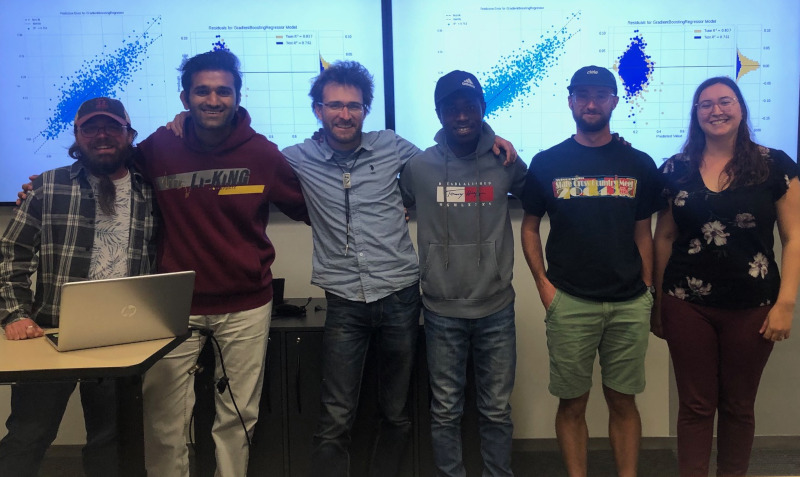
\includegraphics[height=5cm]{2022-10-14_ML_group_meeting.jpg} \\
}

\date{}

\maketitle

\section{Introduction: two common questions in collaborations involving scientific applications of machine learning}

\begin{frame}
  \frametitle{Learning two different functions using two data sets}
  Figure from chapter by Hocking TD, \textit{Introduction to machine
    learning and neural networks} for book \textit{Land Carbon Cycle
    Modeling: Matrix Approach, Data Assimilation, and Ecological
    Forecasting} edited by Luo Y (Taylor and Francis, 2022).
  \begin{center}
  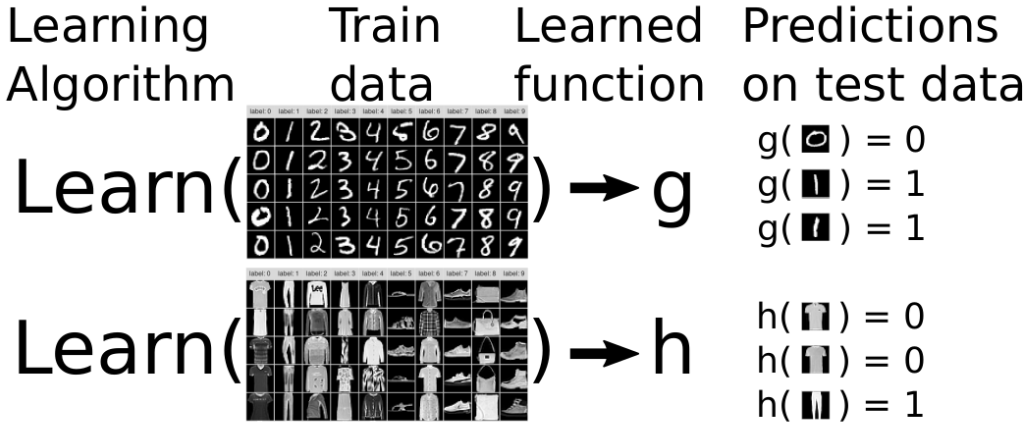
\includegraphics[width=\textwidth]{figure-learn-digits-clothing}
\end{center}
  \textbf{Learn} is a learning algorithm, which outputs
  $g$ and $h$.

  Q: what happens if you do
    $g(
\includegraphics[height=1cm]{fashion-mnist-boot})$, or
    $h(
\includegraphics[height=1cm]{mnist-0})$?
\end{frame}

\begin{frame}
  \frametitle{Train on one subset and accurately predict on another?} 
  \begin{itemize}
  \item This is a question about \textbf{generalization}: how accurate
    is the learned function on a new/test data subset which is
    \textbf{qualitatively different} in some respect?
  \item ``Very accurate'' if test data are similar enough to train data (best case is i.i.d. = independent and identically distributed)
  \item What if you do
    $g(
\includegraphics[height=1cm]{fashion-mnist-boot})$, or
    $h(
\includegraphics[height=1cm]{mnist-0})$? (\textbf{different pattern})
  \item Predicting childhood autism (Lindly \emph{et al.}), train on
    one year of surveys, test on another. (\textbf{different time periods})
  \item Predicting carbon emissions (Aslam \emph{et al.}), train on
    one city, test on another. (\textbf{different geographic regions})
  \item Predicting presence of trees/burn in satellite imagery
    (Shenkin \emph{et al.}, \emph{Thibault} \emph{et al.}), train on
    one geographic area/image, test on another. (\textbf{different geographic regions})
  \item Predicting fish spawning habitat in sonar imagery (Bodine
    \emph{et al.}), train on one river, test on another. (\textbf{geographic regions})
  \item But how do we check if ``very accurate'' in each situation?
  \end{itemize}
\end{frame}

\begin{frame}
  \frametitle{How to deal with class imbalance?}
  \begin{itemize}
  \item In binary classification, standard learning algorithms can yield sub-optimal prediction accuracy if train data have imbalanced labels.
  \item Predicting childhood autism (Lindly \emph{et al.}), 3\% autism, 97\% not.
  \item Predicting presence of trees/burn in satellite imagery
    (Shenkin \emph{et al.}, \emph{Thibault} \emph{et al.}), small
    percent of trees in deserts of Arizona, small percent of burned
    area out of total forested area in Quebec.
  \item Predicting fish spawning habitat in sonar imagery (Bodine
    \emph{et al.}), small percent of suitable spawning habitat, out of
    total river bed.
  \item How do we adapt our learning algorithm, to handle the class imbalance?
  \end{itemize}
\end{frame}

\section{Train on one subset and accurately predict on another? \\ SOAK: Same/Other/All K-fold cross-validation for estimating similarity of patterns in data subsets (arXiv:2410.08643)}

\begin{frame}
  \frametitle{Example data with subsets: predicting childhood autism}

  \begin{itemize}
  \item Collaboration with Lindly \emph{et al.}
  \item Downloaded National Survey of Children's Health (NSCH) data,
    years 2019 and 2020, from
    \url{http://www2.census.gov/programs-surveys/nsch}
  \item One row per person ($N=46,010$ rows), one column per survey question ($D=366$ columns). 
  \item Output/label column is diagnosis with Autism\\
    (binary classification, yes or no),\\
    can we predict it using the 365 inputs/features?
  \item 18,202 rows for 2019; 27,808 rows for 2020.
  \end{itemize}
  Proposed SOAK algorithm is a generalization of standard K-fold cross-validation, that can be used to answer two related questions:
  \begin{itemize}
  \item Can we train on one year, and accurately predict on another?
  \item Can we get a more accurate model by combining data from different years?
  \end{itemize}

\end{frame} 

\begin{frame}
  \frametitle{$K$-fold cross-validation: a standard algorithm used to estimate prediction accuracy in machine learning}

  \begin{itemize}
  \item $K=3$ folds shown in figure below, meaning three different
    models trained, and three different prediction/test accuracy rates
    computed.
  \item It is important to use several train/test splits, so we can
    see if there are statistically significant differences between
    algorithms.
  \end{itemize}

  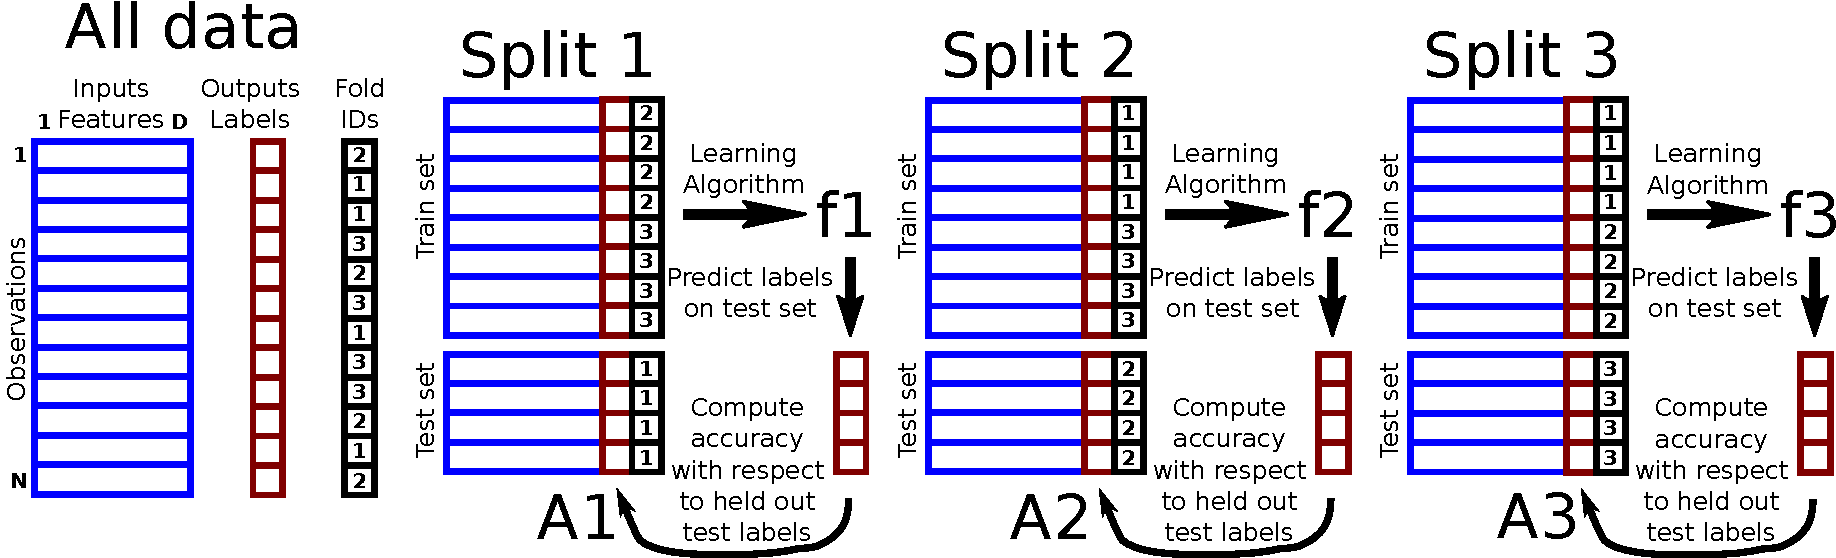
\includegraphics[width=\textwidth]{drawing-cross-validation.pdf}

  \small Hocking TD \emph{Intro. to machine learning and neural
    networks} (2022).
\end{frame}


\begin{frame}
  \frametitle{Proposed SOAK algorithm (Autism data example)}
  \begin{itemize}
  \item Example: childhood autism prediction data set.
  \item Subsets of interest are years, which can be represented by
    adding a new column to the data table.
  \end{itemize}
  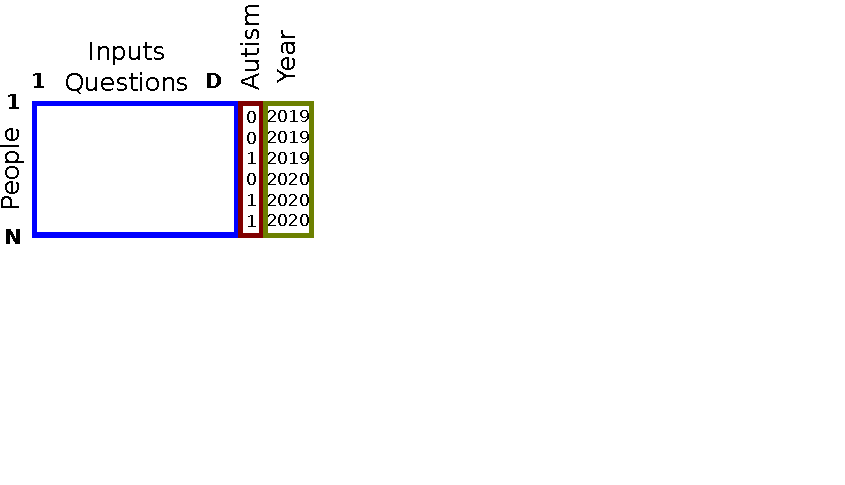
\includegraphics[width=\textwidth]{drawing-cv-same-other-years-1.pdf}
\end{frame}

\begin{frame}
  \frametitle{Proposed SOAK algorithm (Autism data example)}
  \begin{itemize}
  \item Train subset same as test (=regular $K$-fold CV on 2020).
    \item Do we get a more or less accurate model than this baseline Same model? (if we train on Other/All years)
  \end{itemize}
  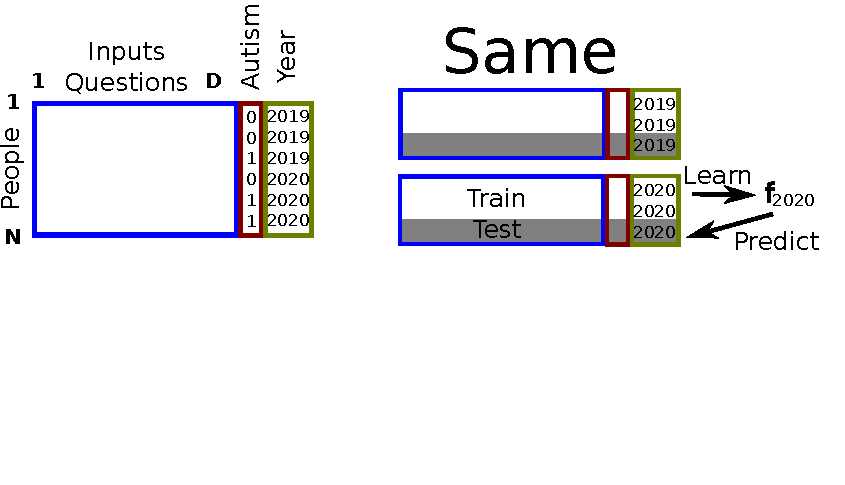
\includegraphics[width=\textwidth]{drawing-cv-same-other-years-2.pdf}
\end{frame}

\begin{frame}
  \frametitle{Proposed SOAK algorithm (Autism data example)}
  \begin{itemize}
  \item Test subset fixed (2020), train on other subset/year (2019).
    \item Can we train on one year, and accurately predict on another? Compare Same/Other test error.
  \end{itemize}
  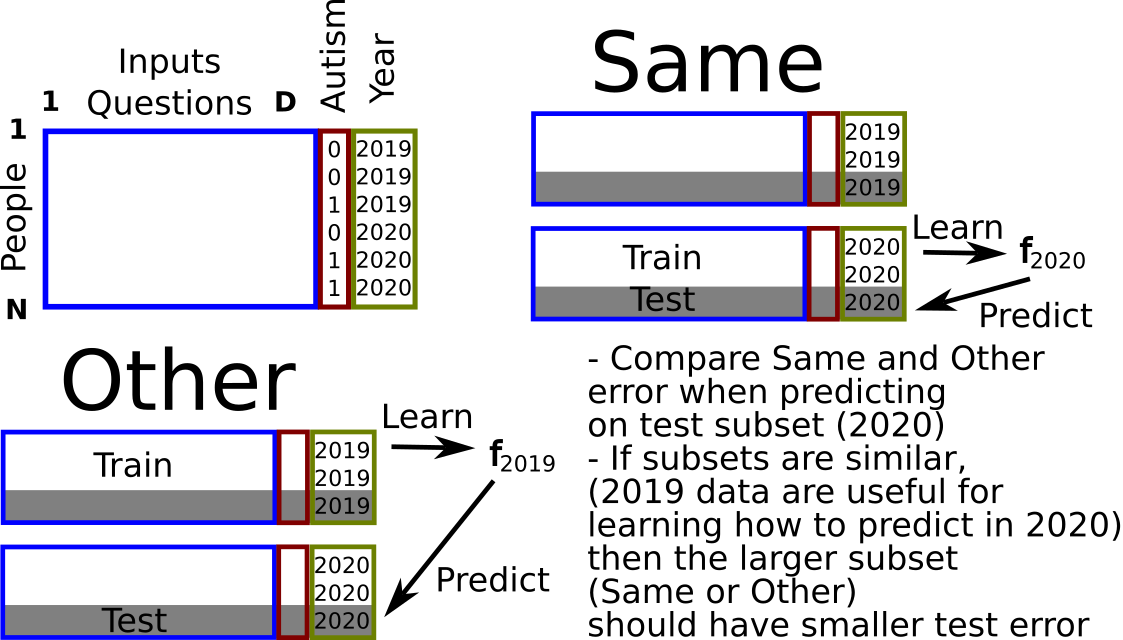
\includegraphics[width=\textwidth]{drawing-cv-same-other-years-ann}
\end{frame}

\begin{frame}
  \frametitle{Proposed SOAK algorithm (Autism data example)}
  \begin{itemize}
  \item Train set includes data from both subsets/years (2019, 2020).
    \item Can we get a more accurate model by combining data from
      different years? Compare Same/All test error.
  \end{itemize}
  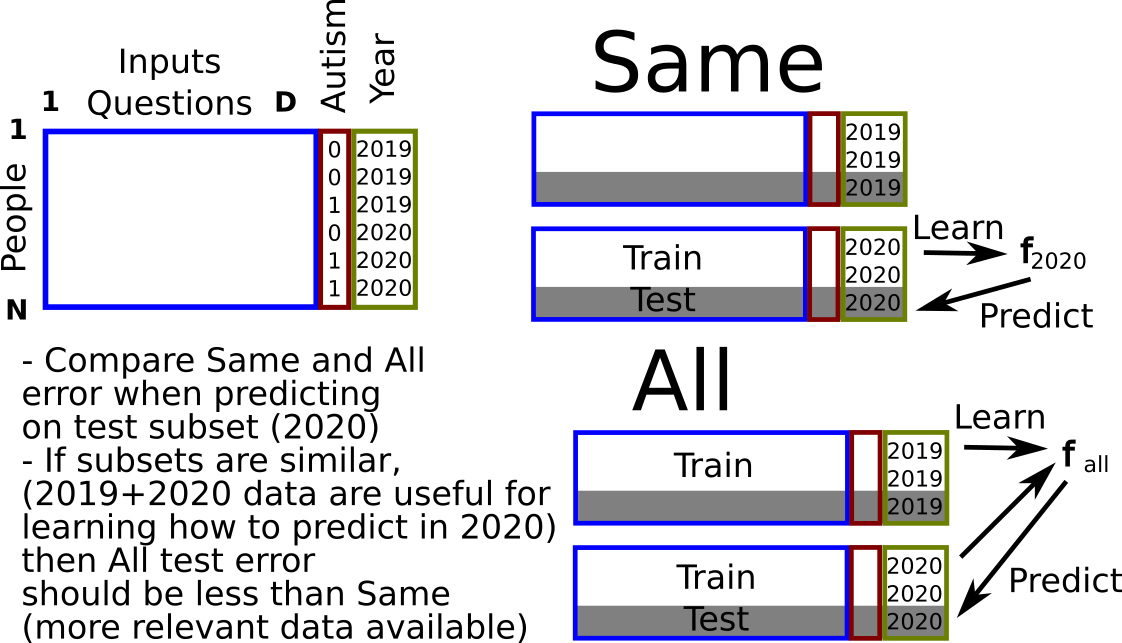
\includegraphics[width=\textwidth]{drawing-cv-same-all-years-ann}
\end{frame}

\begin{frame}
  \frametitle{Proposed SOAK algorithm (generic data)}
  \begin{itemize}
  \item Key new idea is \textbf{subset} column in data table.
  \item Example: $K=3$ folds, two subsets (A/B).
  \item Compute test error for each fold (1/2/3) and subset (A/B).
  \end{itemize}
  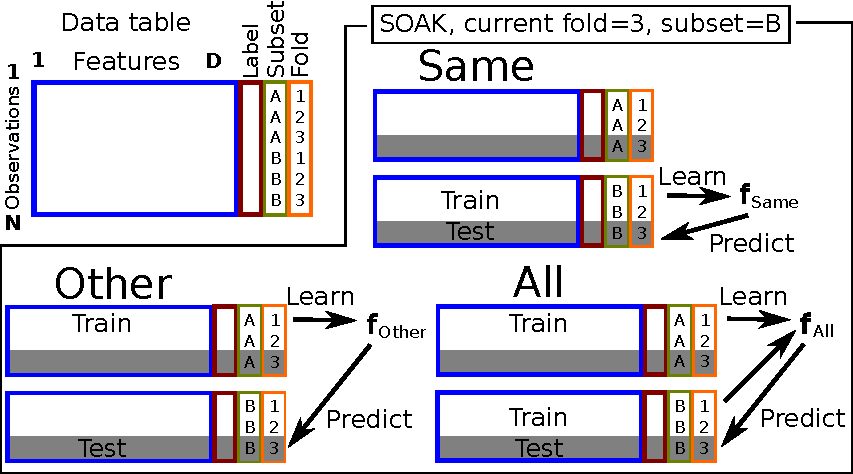
\includegraphics[width=\textwidth]{drawing-cv-same-other-generic}
\end{frame}

% \begin{frame}
%   \frametitle{Proposed SOAK algorithm, interpretation/expectations}

%   For a fixed test set from one subset:
   
%   If subsets have similar learnable/predictable patterns,
%   \\(this is a weaker condition than i.i.d.)
%   \begin{description}
%   \item[All] should be most accurate.
%   \item[Same/Other] should be less accurate, because there is less
%     data available (if more data in Other than in Same, then Other should be
%     more accurate than Same, etc).
%   \end{description}

%   If subsets have different learnable/predictable patterns,
%   \begin{description}
%   \item[Same] should be most accurate.
%   \item[Other] should be substantially less accurate.
%   \item[All] accuracy should be between Same and Other.
%   \end{description}
%   \begin{itemize}
%     \item Can we train on one year, and accurately predict on another? Compare Same/Other test error.
%     \item Can we get a more accurate model by combining data from
%       different years? Compare Same/All test error.
%   \end{itemize}

% \end{frame}

\begin{frame}
  \frametitle{Proposed SOAK algorithm new to ML frameworks}
  \small
  \begin{itemize}
  \item ML frameworks like scikit-learn and mlr3 implement cross-validation with \textbf{groups} of samples that must stay together when splitting.
  \item For example (below), satellite image segmentation, trees vs background, Shenkin \emph{et al.}: samples=pixels, grouped by polygon, SOAK subsets are geographical regions (NW, NE, S).
  \item SOAK: good predictions on one test \textbf{subset},
    after training on Same/Other/All subsets? (can use together with groups)
  \end{itemize}
  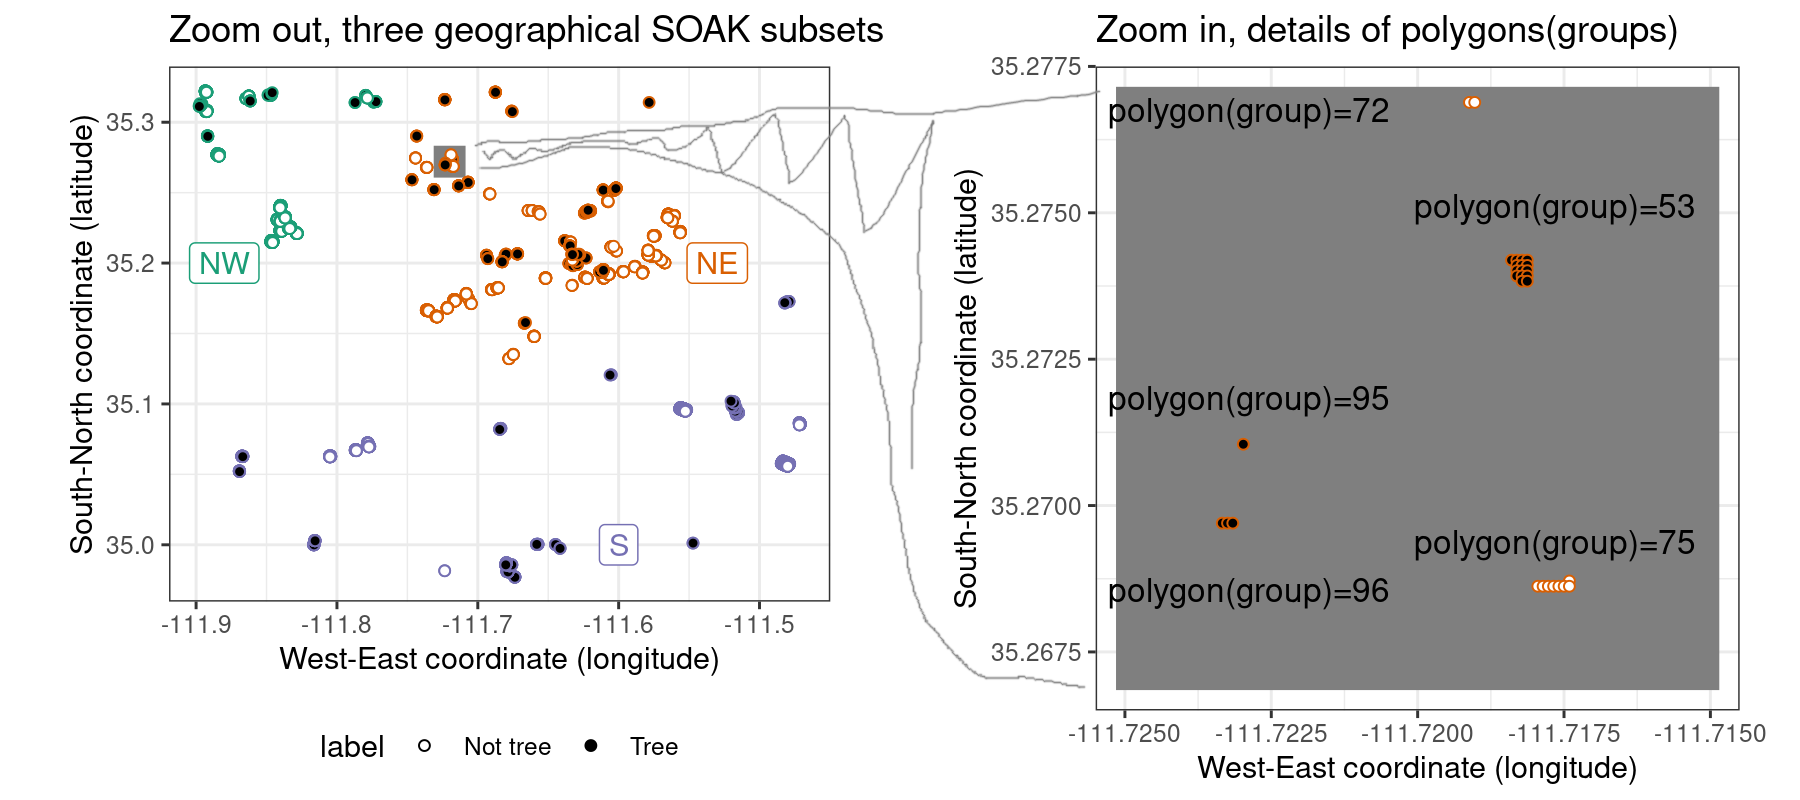
\includegraphics[width=\textwidth]{figure-aztrees}
\end{frame}


\begin{frame}
  \frametitle{ImagePair data: train on MNIST and accurately predict on MNIST variants?}

  \begin{itemize}
  \item Expect: $g(
\includegraphics[height=1cm]{fashion-mnist-boot})$ and
    $h(
\includegraphics[height=1cm]{mnist-0})$ are not accurate.
  \item But train on MNIST, predict on EMNIST\_rot (upright digits) should be
    possible, right? (Vote!) Let's use SOAK to find out!
  \item Create three new IPair data sets by combining MNIST with variants:
    EMNIST, EMNIST\_rot, FashionMNIST.
  \item Each data set has two subsets: MNIST/variant.
 \end{itemize}

  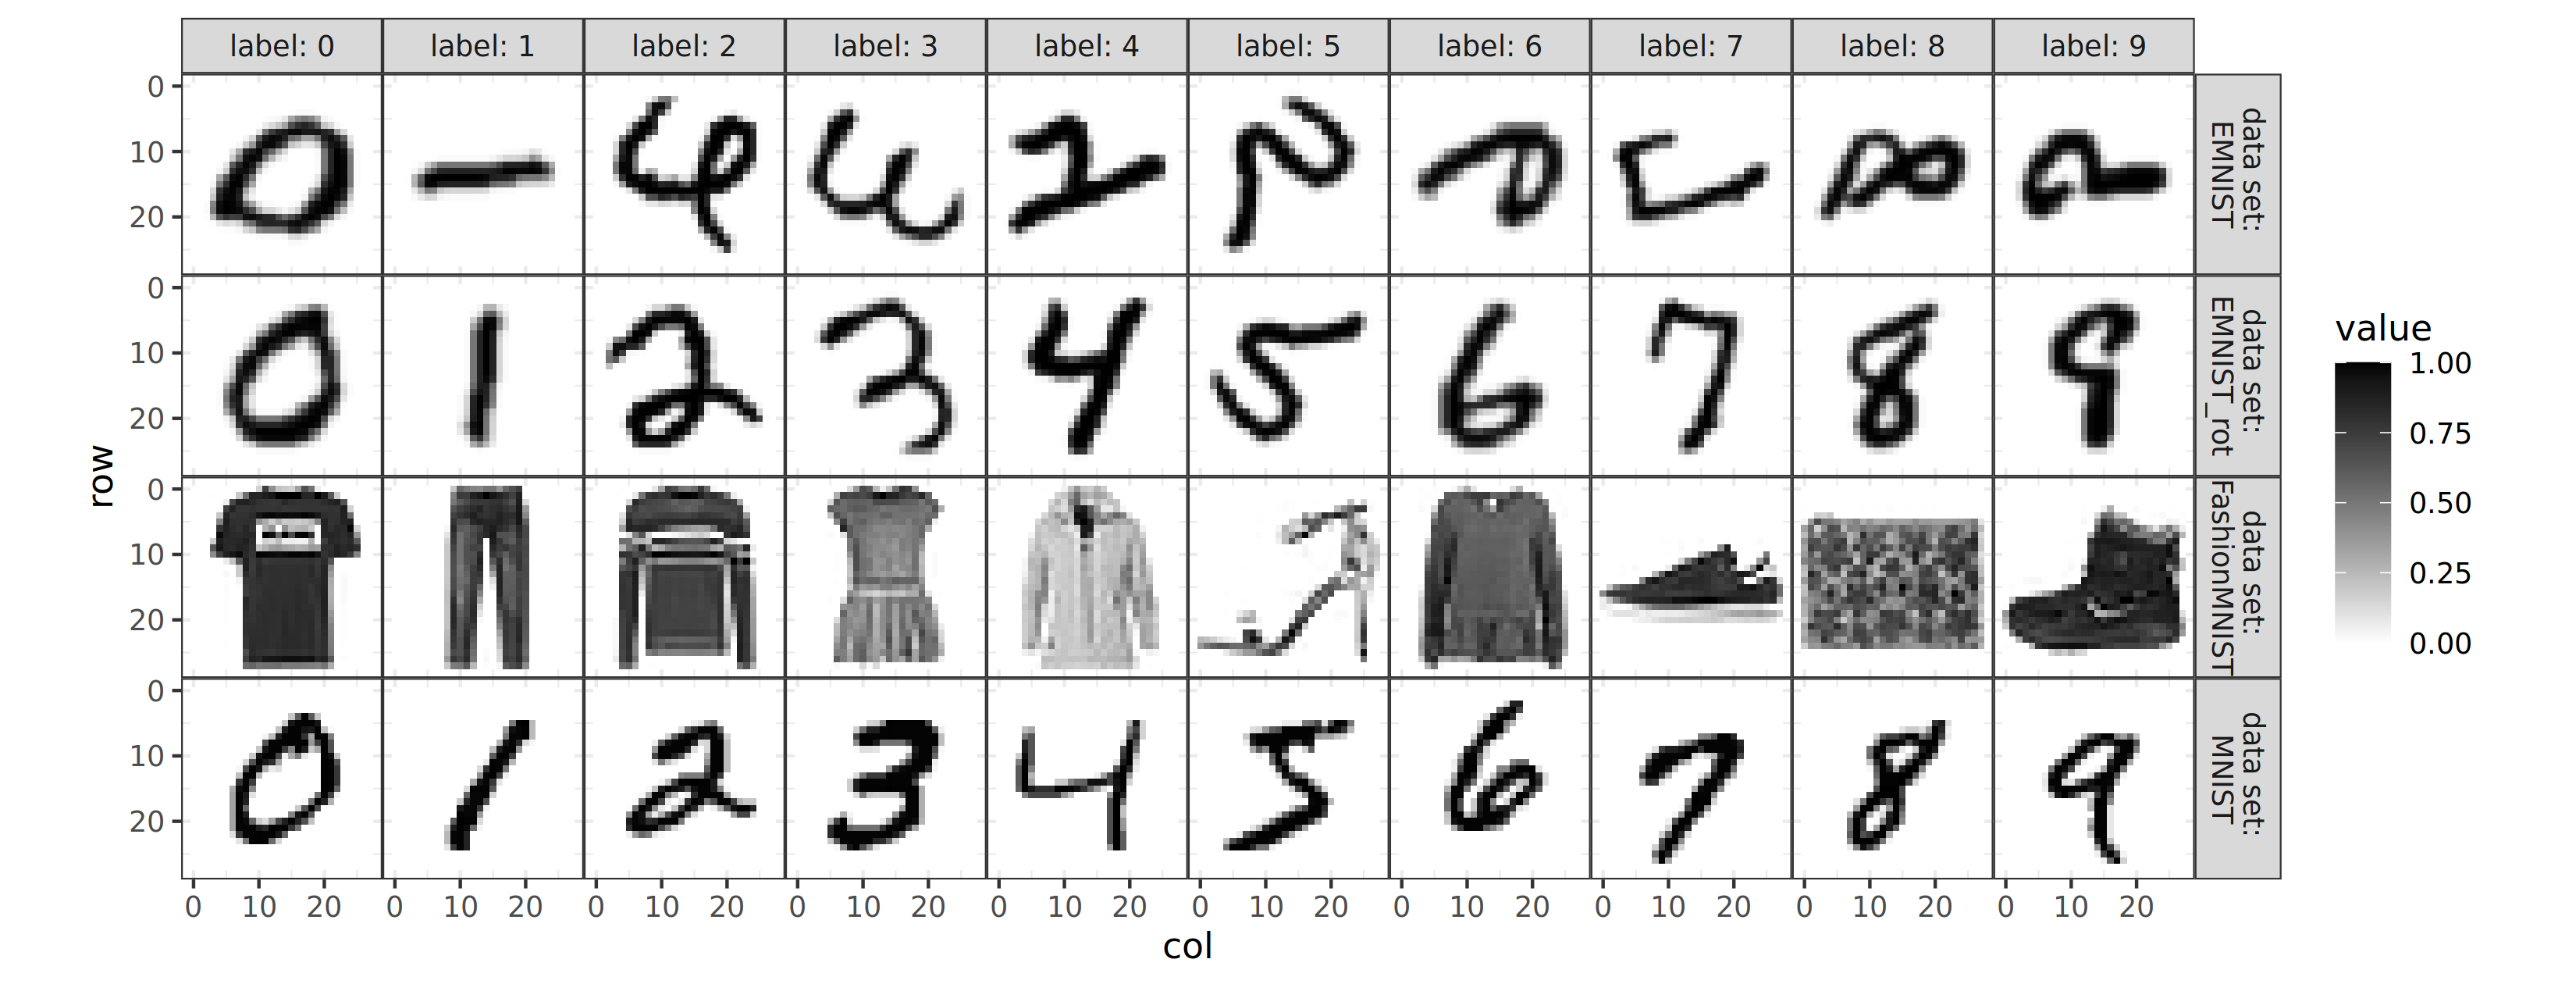
\includegraphics[width=\textwidth]{data_Classif_MNIST_other_1.png}
\end{frame}

\begin{frame}
  \frametitle{SOAK for MNIST+FashionMNIST (IPair\_Fashion data set)}

  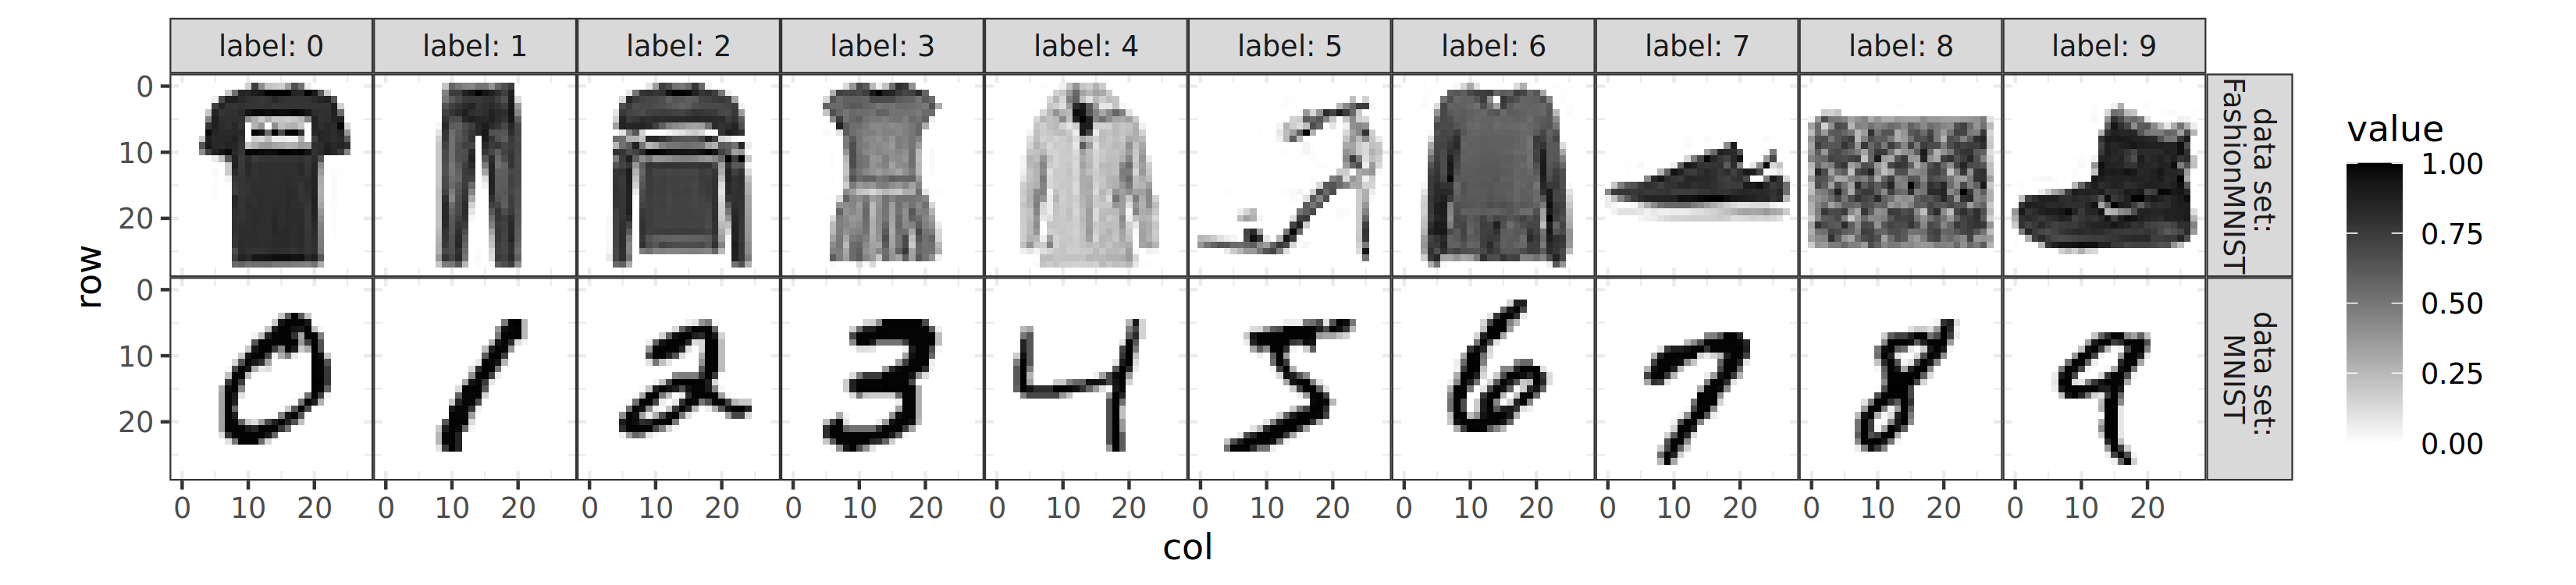
\includegraphics[width=\textwidth]{data_Classif_MNIST_other_FashionMNIST.png}
  
  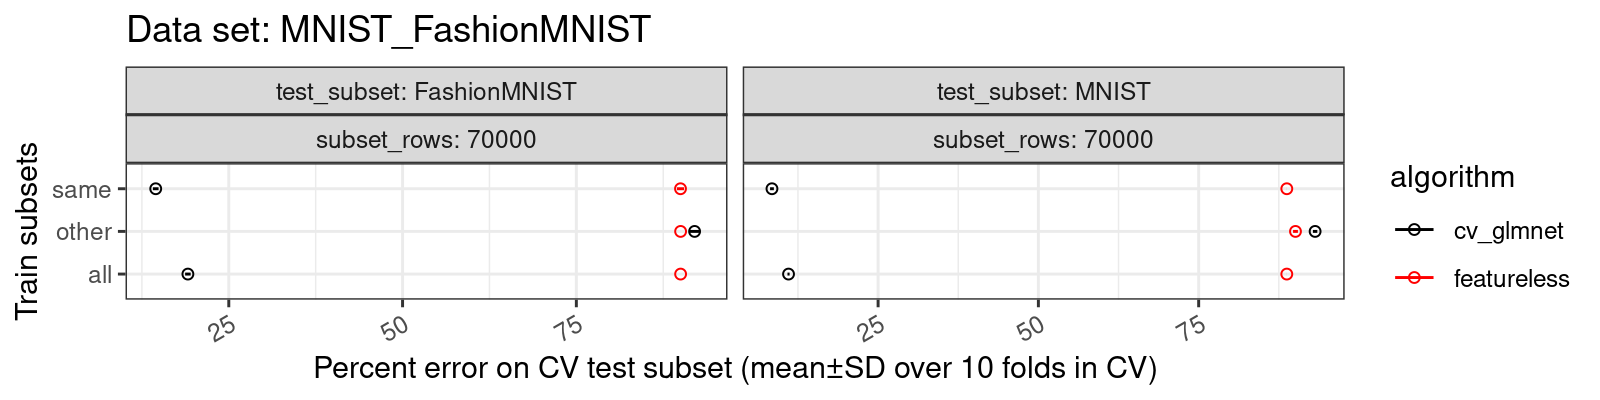
\includegraphics[width=\textwidth]{MNIST_FashionMNIST_error_glmnet_featureless_mean_SD.png}
  \begin{itemize}
  \item \textbf{cv\_glmnet} is L1-regularized linear model.
  \item \textbf{featureless} baseline always predicts most frequent class.
  \item \textbf{Other cv\_glmnet} has greater test error than
    \textbf{featureless}.
  \item The patterns in the two subsets are too different for \textbf{Other cv\_glmnet} to learn
    anything useful for prediction. (expected)
  \end{itemize}
\end{frame}

\begin{frame}
  \frametitle{SOAK for MNIST+EMNIST (IPair\_E data set)}

  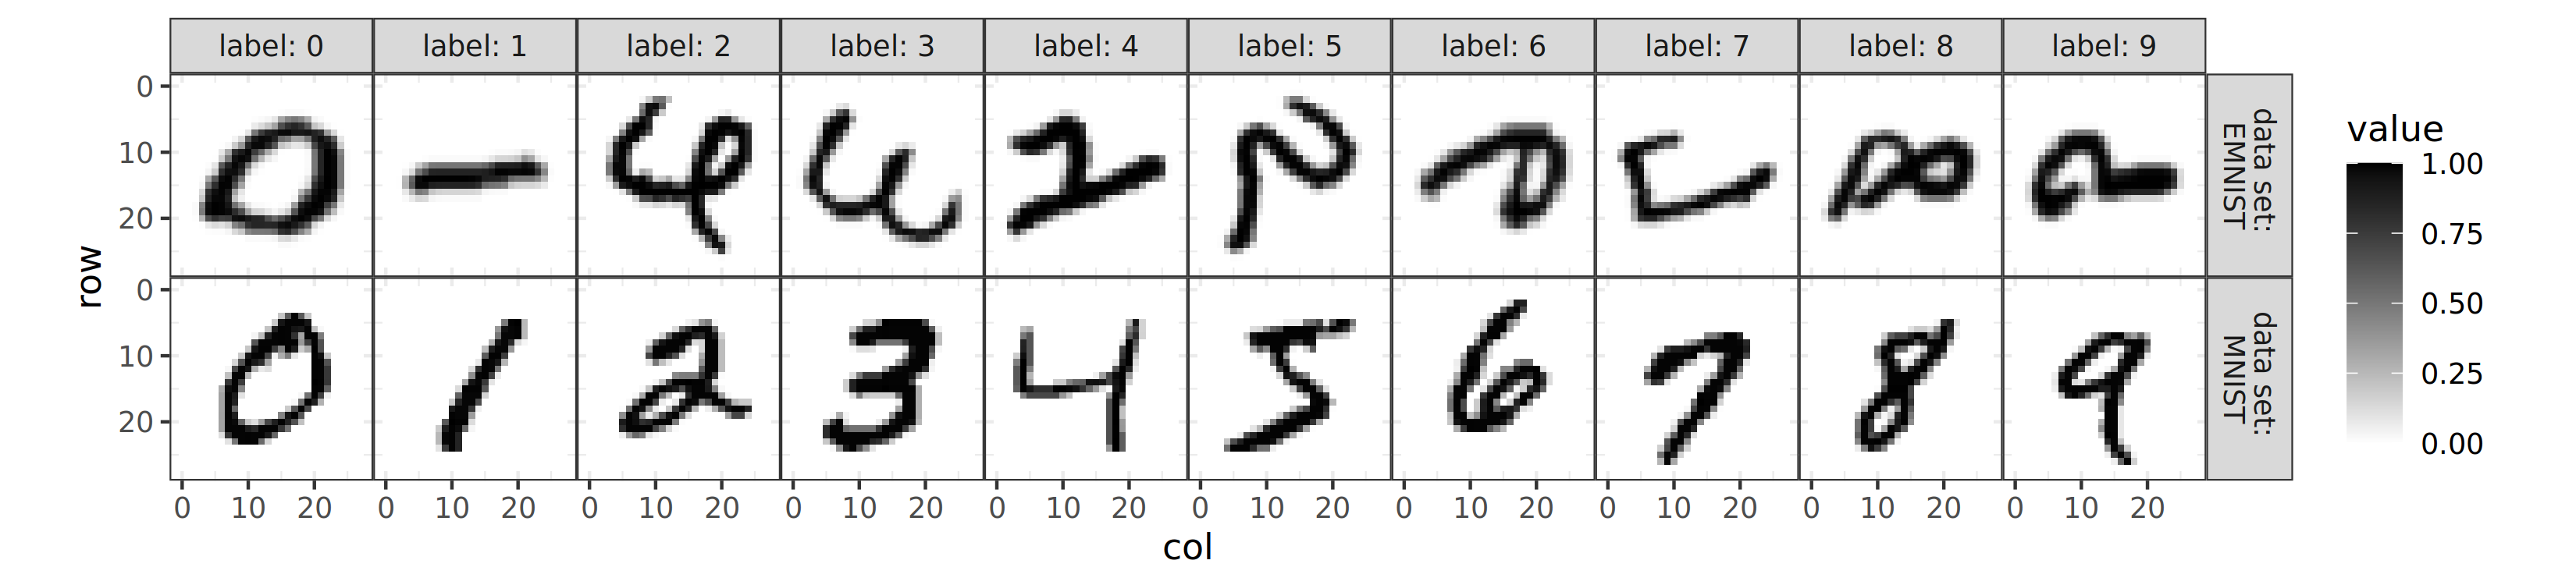
\includegraphics[width=\textwidth]{data_Classif_MNIST_other_EMNIST.png}
  
  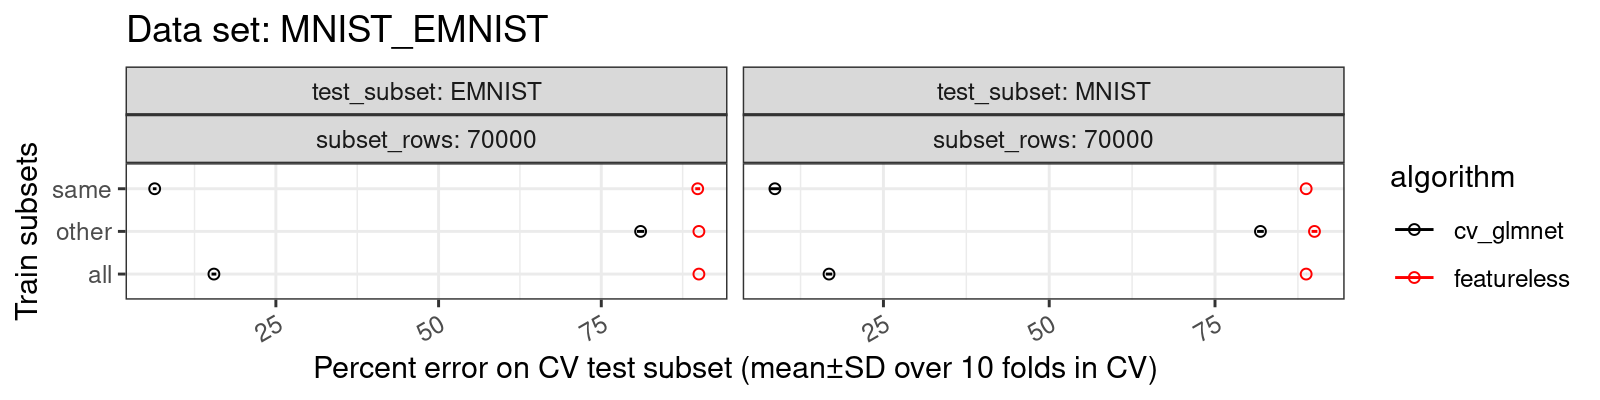
\includegraphics[width=\textwidth]{MNIST_EMNIST_error_glmnet_featureless_mean_SD.png}
  \begin{itemize}
  \item \textbf{Other cv\_glmnet} has significantly smaller test error
    than \textbf{featureless}, so linear model learns something that useful for predicting on the other subset.
  \item But since \textbf{Other} error rate is much larger than
    \textbf{Same}, clearly the pattern is very different between
    MNIST/EMNIST.
  \end{itemize}
\end{frame}

\begin{frame}
  \frametitle{SOAK for MNIST+EMNIST\_rot (IPair\_E\_rot data set)}

  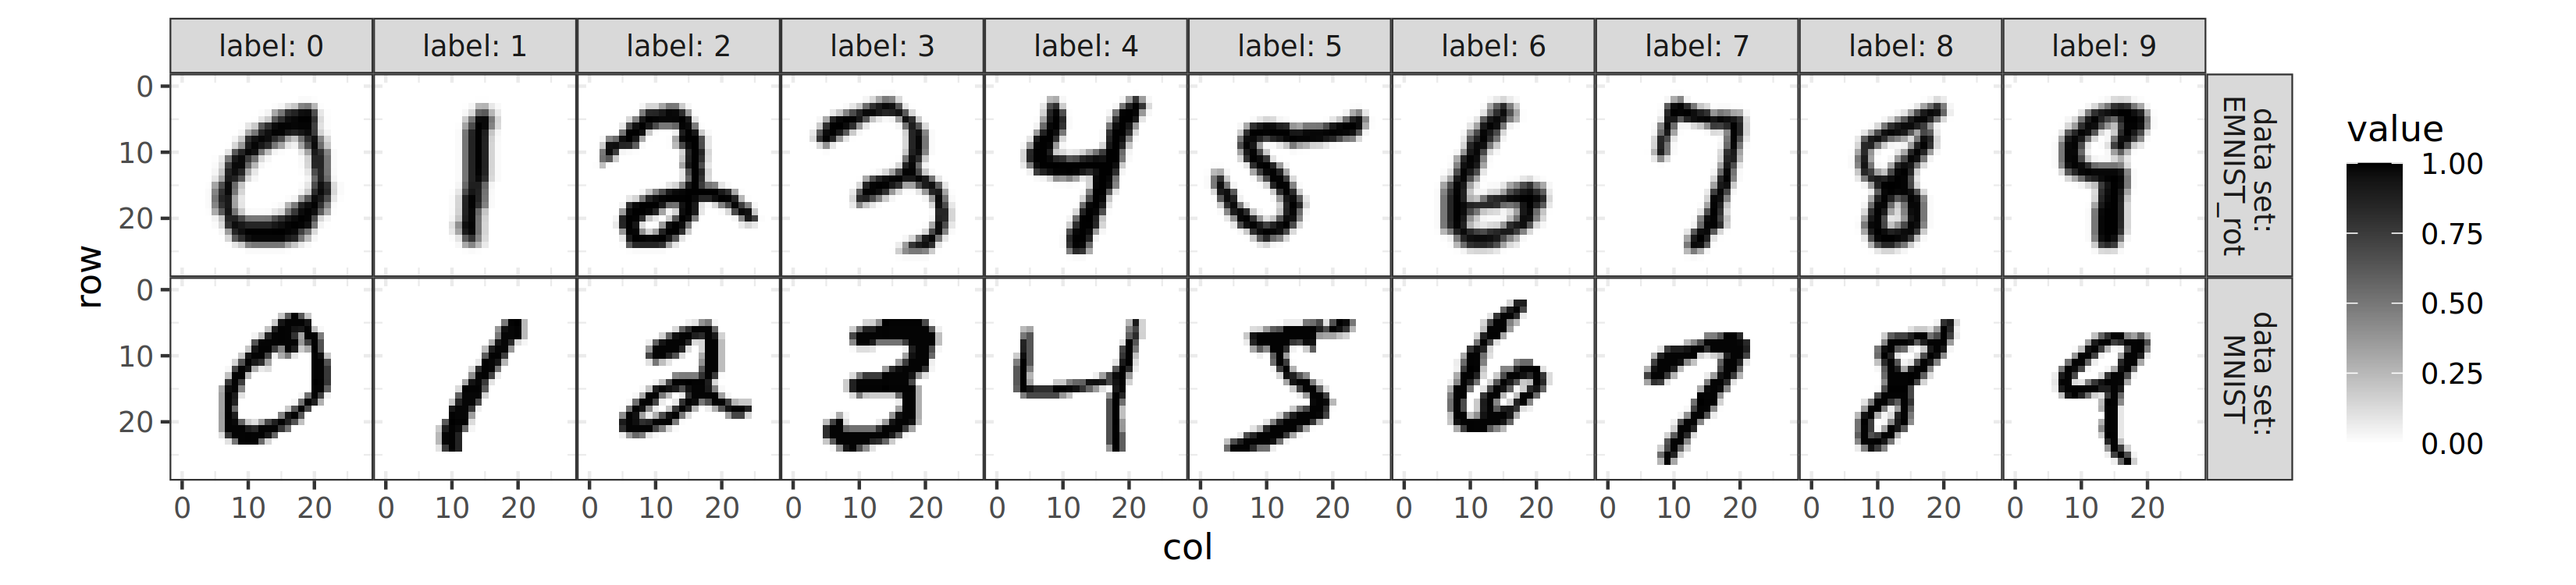
\includegraphics[width=\textwidth]{data_Classif_MNIST_other_EMNIST_rot.png}
  
  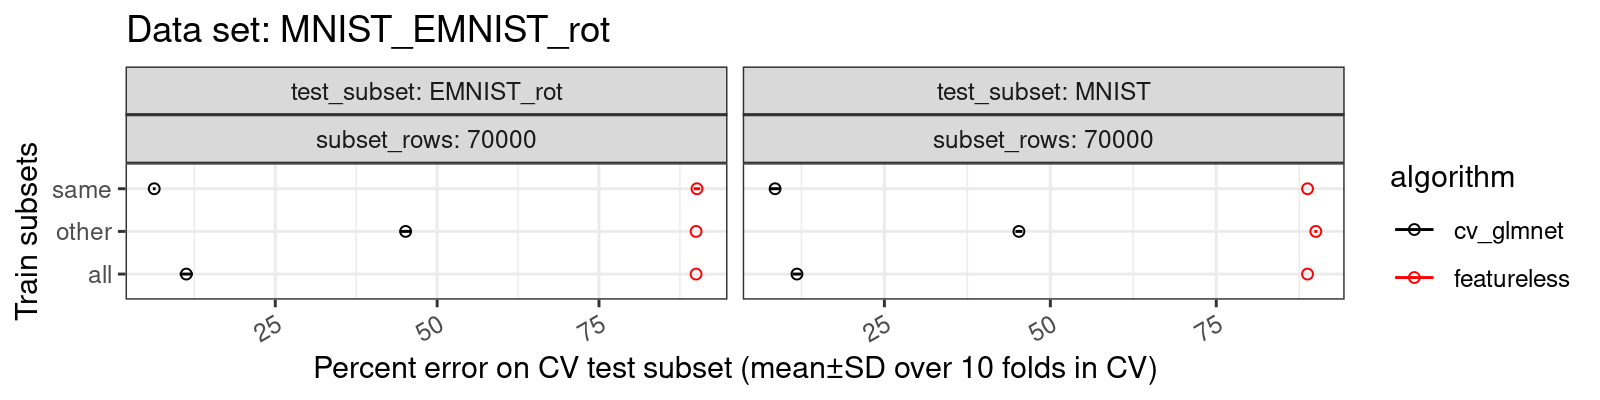
\includegraphics[width=\textwidth]{MNIST_EMNIST_rot_error_glmnet_featureless_mean_SD.png}
  \begin{itemize}
  \item \textbf{Other cv\_glmnet} has even smaller test error,
    indicating even more similarity between MNIST and EMNIST\_rot data
    sets.
  \item But \textbf{Other/All} test error are still not as small as \textbf{Same}.
  \item Significant difference between patterns learnable/predictable
    by linear model in MNIST/EMNIST\_rot. (surprising)
  \end{itemize}
\end{frame}

\begin{frame}
  \frametitle{Benchmark data with pre-defined train/test subsets}
  \begin{itemize}
  \item Machine learning researchers evaluate new algorithms using
    benchmark data sets, which sometimes have pre-defined train/test
    subsets.
% > meta.dt[data.name=="MNIST"]
%    data.name memory.kb  rows n.groups              group.tab group.small.name
%       <char>     <int> <int>    <int>                 <char>           <char>
% 1:     MNIST    429712 70000        2 test=10000;train=60000             test
%    group.small.N group.large.name group.large.N label.small.name label.small.N
%            <int>           <char>         <int>           <char>         <int>
% 1:         10000            train         60000                0          6903
%    label.large.name label.large.N features classes min.rows  test train test%
%              <char>         <int>    <int>   <int>    <int> <int> <int> <int>
% 1:                9          6958      784      10      892 10000 60000    14 
  \item For example KMNIST is an image classification data set with \\
    60,000 images in a pre-defined train subset, and \\
    10,000 images in a pre-defined test subset.
% > meta.dt[data.name=="spam"]
%    data.name memory.kb  rows n.groups            group.tab group.small.name
%       <char>     <int> <int>    <int>               <char>           <char>
% 1:      spam      2078  4601        2 test=1536;train=3065             test
%    group.small.N group.large.name group.large.N label.small.name label.small.N
%            <int>           <char>         <int>           <char>         <int>
% 1:          1536            train          3065                0          2788
%    label.large.name label.large.N features classes min.rows  test train test%
%              <char>         <int>    <int>   <int>    <int> <int> <int> <int>
% 1:                1          1813       57       2      595  1536  3065    33
  \item STL10 is another image classification data set with \\
    5000 images in a pre-defined train subset, and \\
    8000 images in a pre-defined test subset.
  \item Are the learnable/predictable patterns in the pre-defined train/test subsets
    similar? (expected if random sampling was used to create pre-defined subsets)
  \item Use pre-defined train/test subsets in SOAK, to see if patterns are learnable/predictable across pre-defined subsets.
  \end{itemize}
\end{frame}

\begin{frame}
  \frametitle{Benchmark data with pre-defined train/test subsets}
  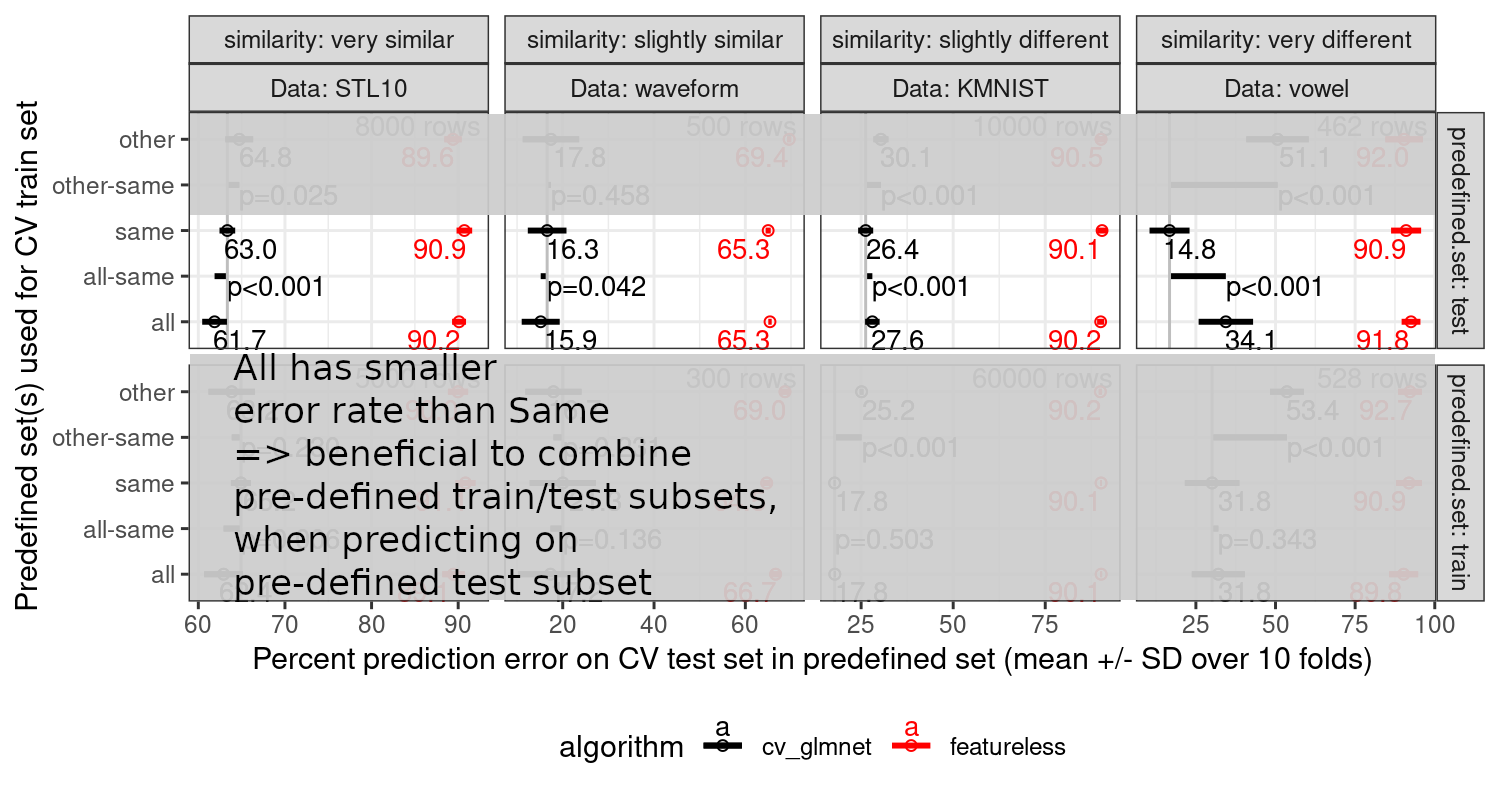
\includegraphics[width=\textwidth]{data_Classif_batchmark_registry_glmnet_featureless_mean_sd_similar_all_test}
\end{frame}

\begin{frame}
  \frametitle{Benchmark data with pre-defined train/test subsets}
  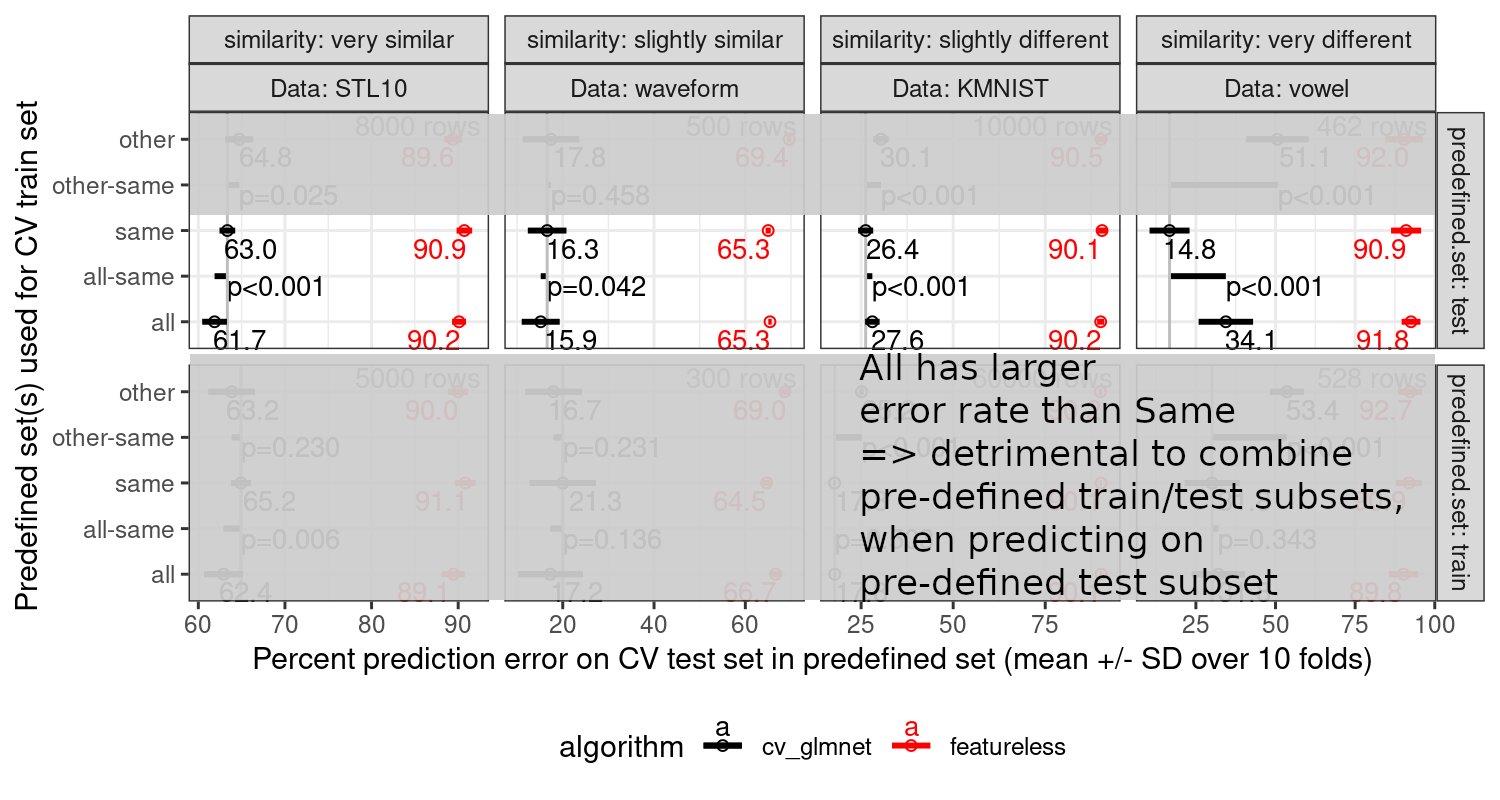
\includegraphics[width=\textwidth]{data_Classif_batchmark_registry_glmnet_featureless_mean_sd_different_all_test}
\end{frame}

\begin{frame}
  \frametitle{Benchmark data with pre-defined train/test subsets}
  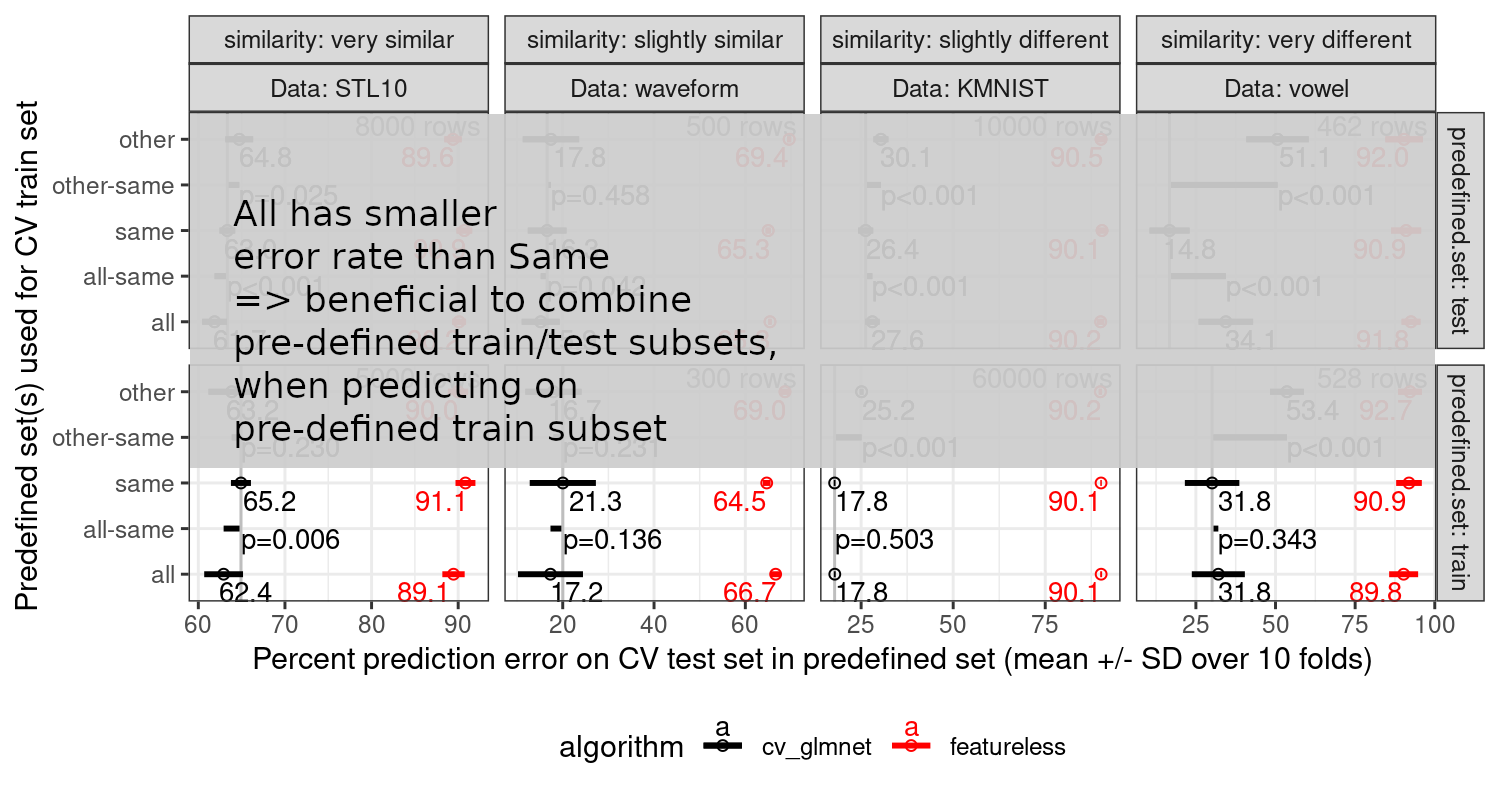
\includegraphics[width=\textwidth]{data_Classif_batchmark_registry_glmnet_featureless_mean_sd_similar_all_train}
\end{frame}

\begin{frame}
  \frametitle{Benchmark data with pre-defined train/test subsets}
  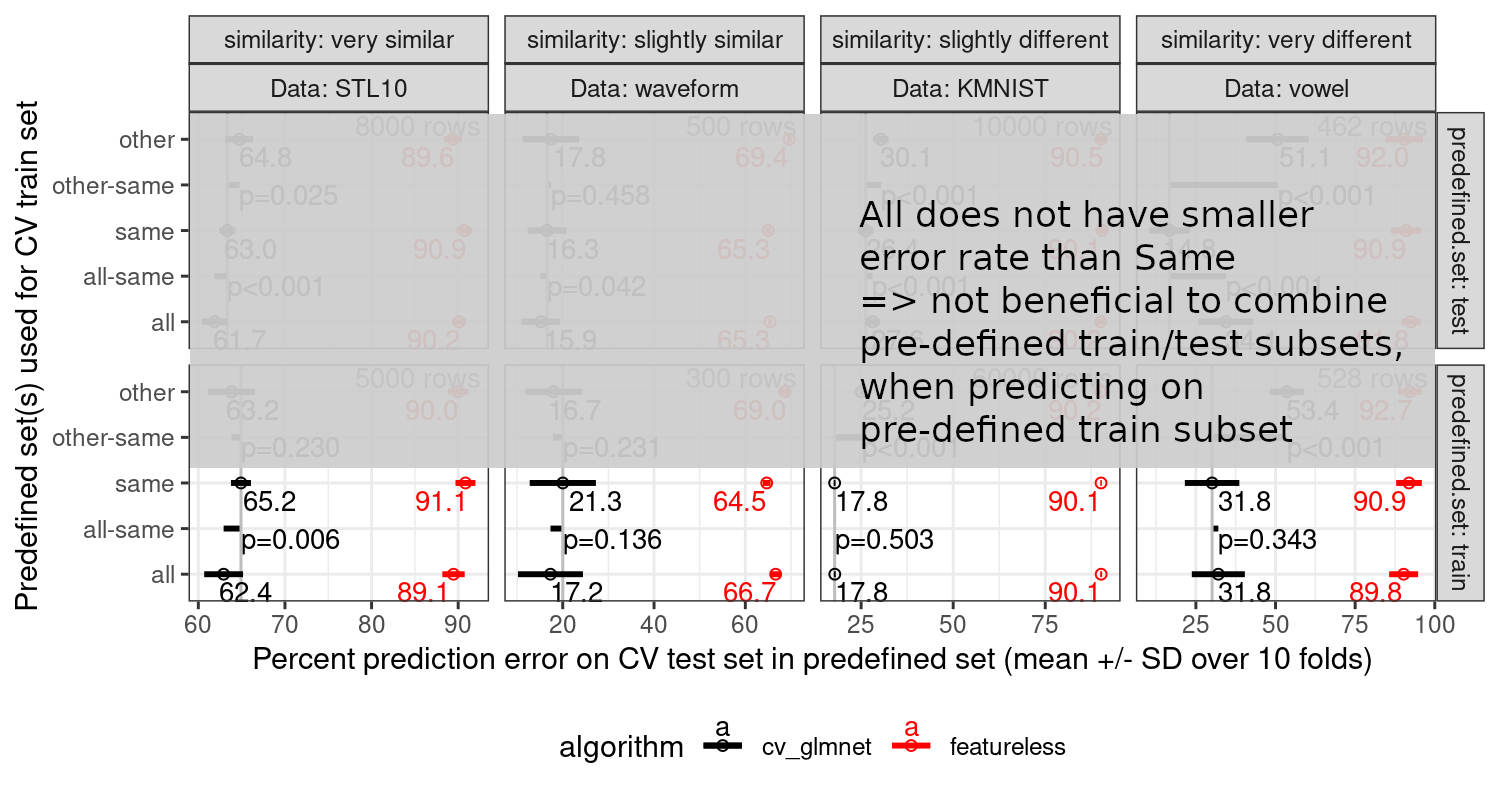
\includegraphics[width=\textwidth]{data_Classif_batchmark_registry_glmnet_featureless_mean_sd_different_all_train}
\end{frame}

\begin{frame}
  \frametitle{Benchmark data with pre-defined train/test subsets}
  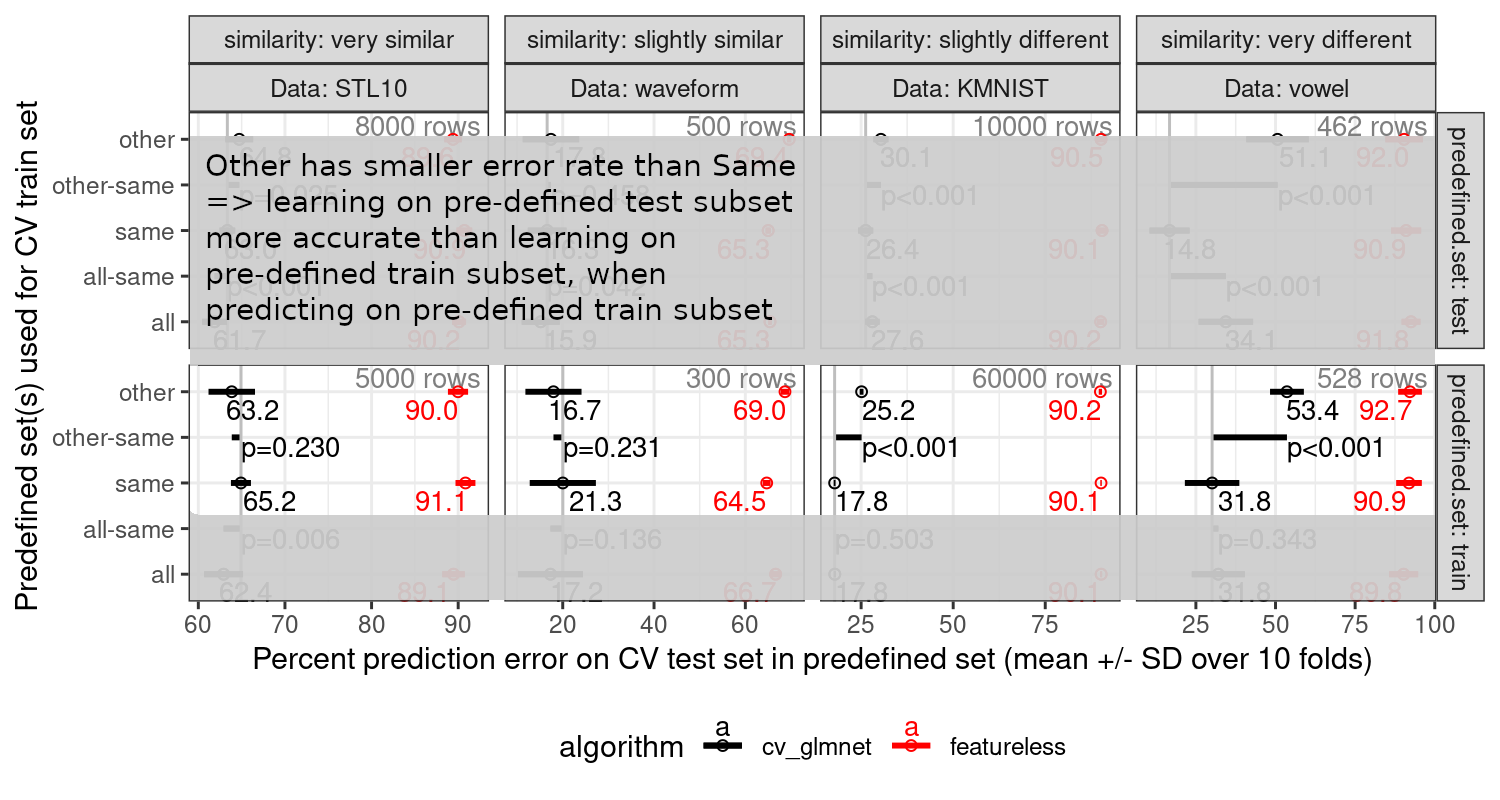
\includegraphics[width=\textwidth]{data_Classif_batchmark_registry_glmnet_featureless_mean_sd_other_similar_train}
\end{frame}

\begin{frame}
  \frametitle{Benchmark data with pre-defined train/test subsets}
  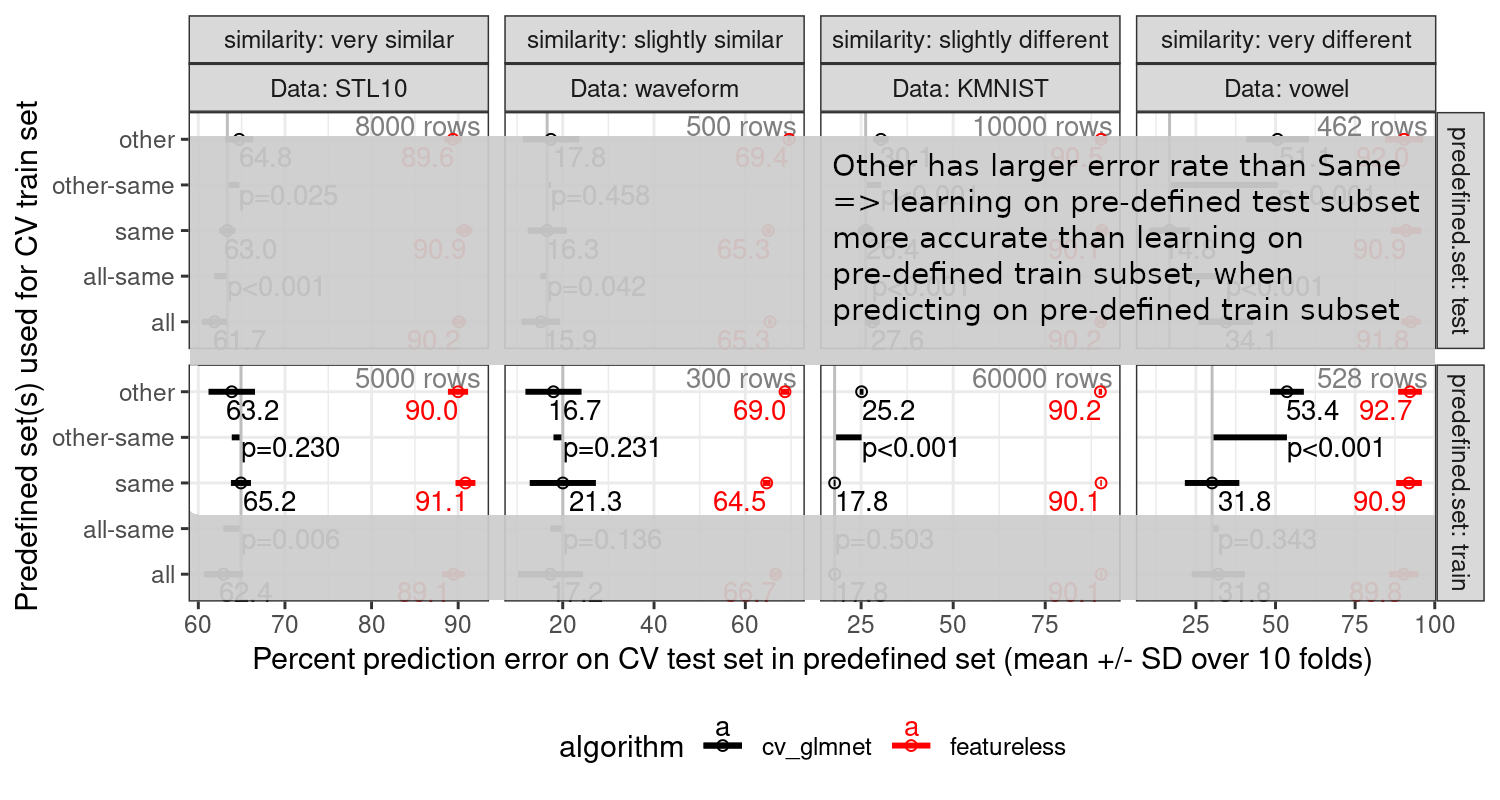
\includegraphics[width=\textwidth]{data_Classif_batchmark_registry_glmnet_featureless_mean_sd_other_different_train}
\end{frame}

\begin{frame}
  \frametitle{Benchmark data with pre-defined train/test subsets}
  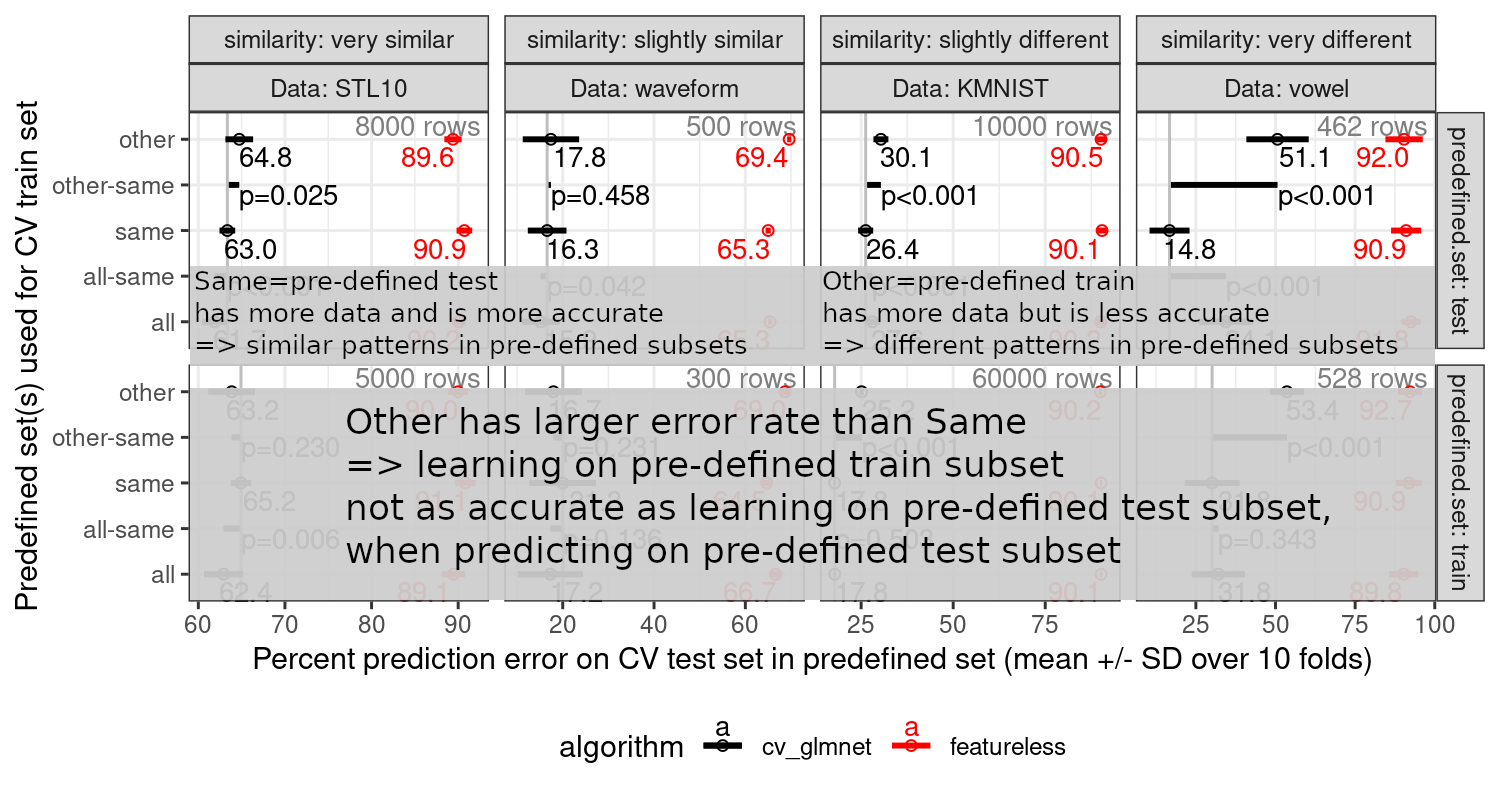
\includegraphics[width=\textwidth]{data_Classif_batchmark_registry_glmnet_featureless_mean_sd_other_test}
\end{frame}
 
\begin{frame}
  \frametitle{Benchmark data with pre-defined train/test subsets}
  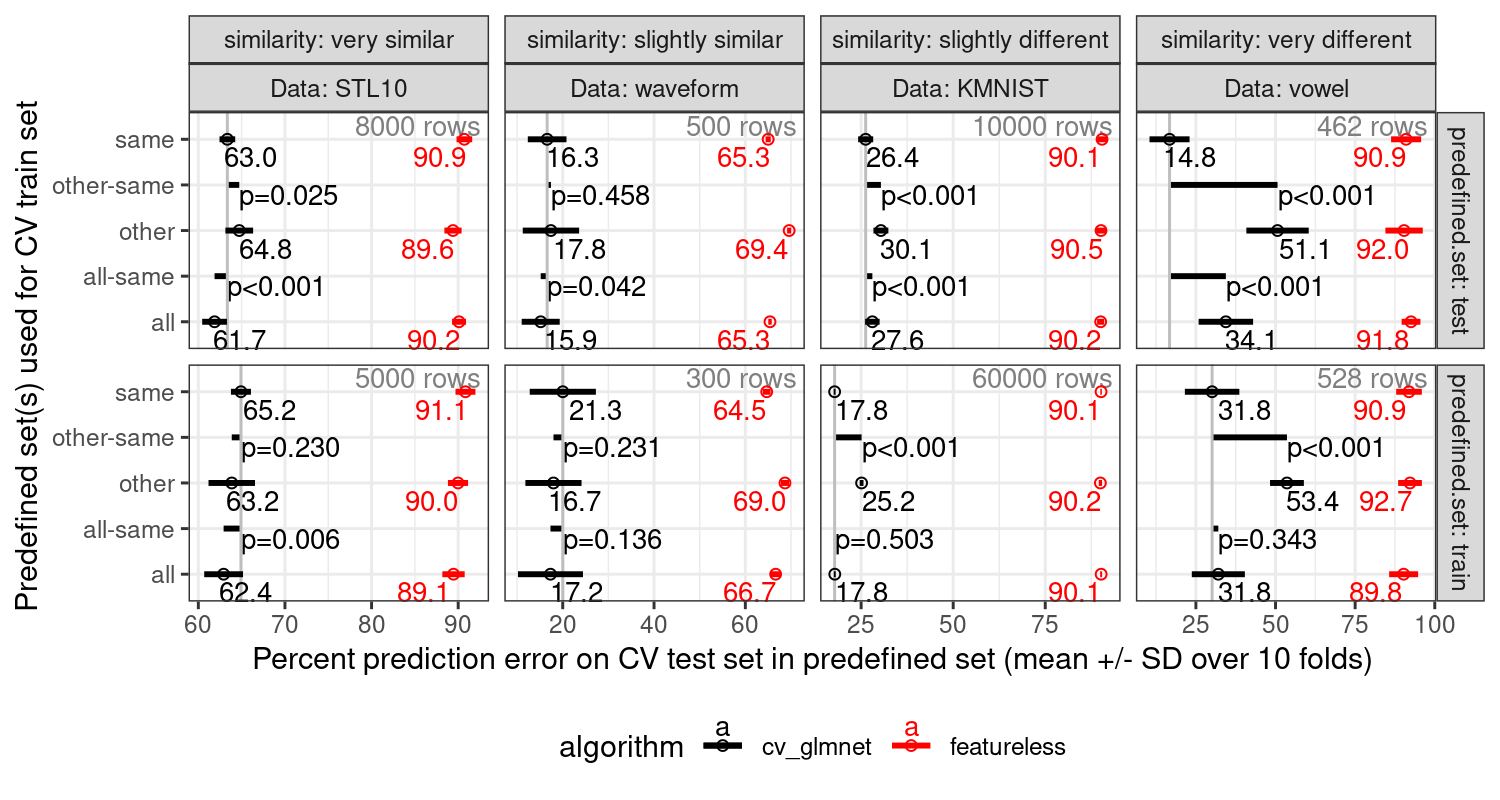
\includegraphics[width=\textwidth]{data_Classif_batchmark_registry_glmnet_featureless_mean_sd}
  \vskip -0.5cm
  \begin{itemize}
  \item Left data sets have similar pre-defined train/test subsets (expected), All error is always less than Same, and Other error is either greater or less than Same, depending on subset sizes. 
  \item Right data sets have different pre-defined train/test subsets (surprising), All error is always greater than or equal to Same, and Other error is always greater than Same.
  \end{itemize}
\end{frame}

\begin{frame}
  \frametitle{20 classification data sets analyzed using SOAK} We
  considered MNIST and variants as subsets (\textbf{ImagePair}),\\
  data from collaborations (\textbf{time/space} subsets), \\
  and benchmark data with
  pre-defined \textbf{train/test} subsets.  \scriptsize
% \begin{tabular}{rlrrrrr}
%   \hline
%  & data.name & rows & features & classes & n.groups & all-same \\ 
%   \hline
% 1 & vowel & 990 &  10 &  11 &   2 & 9.98 \\ 
%   2 & CanadaFires\_downSampled & 1491 &  46 &   2 &   4 & 4.02 \\ 
%   3 & CanadaFires\_all & 4827 &  46 &   2 &   4 & 3.39 \\ 
%   4 & aztrees4 & 5956 &  21 &   2 &   4 & 2.28 \\ 
%   5 & aztrees3 & 5956 &  21 &   2 &   3 & 2.05 \\ 
%   6 & FishSonar\_river & 2815744 &  81 &   2 &   4 & 1.69 \\ 
%   7 & KMNIST & 70000 & 784 &  10 &   2 & 0.87 \\
%   \hline
%   8 & NSCH\_autism & 46010 & 364 &   2 &   2 & -0.03 \\ 
%   9 & MNIST & 70000 & 784 &  10 &   2 & -0.53 \\ 
%   10 & QMNIST & 120000 & 784 &  10 &   2 & -0.70 \\ 
%   11 & spam & 4601 &  57 &   2 &   2 & -0.77 \\ 
%   12 & EMNIST & 70000 & 784 &  10 &   2 & -0.85 \\ 
%   13 & FashionMNIST & 70000 & 784 &  10 &   2 & -0.97 \\ 
%   14 & zipUSPS & 9298 & 256 &  10 &   2 & -1.44 \\ 
%   15 & waveform & 800 &  21 &   3 &   2 & -1.54 \\ 
%   16 & CIFAR10 & 60000 & 3072 &  10 &   2 & -1.77 \\ 
%   17 & STL10 & 13000 & 27648 &  10 &   2 & -1.97 \\ 
%    \hline
% \end{tabular}


\begin{tabular}{rllrrrrr}
  \hline
 & Type & Data & rows & features & classes & subsets & imb. \\ 
  \hline
1 & \tikz\draw[black,fill=black] (0,0) circle (.5ex); ImagePair & IPair\_E & 140000 & 784 & 10 &  2 & 1.0 \\ 
  2 & \tikz\draw[black,fill=black] (0,0) circle (.5ex); ImagePair & IPair\_E\_rot & 140000 & 784 & 10 &  2 & 1.0 \\ 
  3 & \tikz\draw[black,fill=black] (0,0) circle (.5ex); ImagePair & IPair\_Fashion & 140000 & 784 & 10 &  2 & 1.0 \\ 
  4 & \tikz\draw[black,fill=white] (0,0) circle (.5ex); time/space & CanadaFiresA & 4827 & 46 &  2 &  4 & 7.0 \\ 
  5 & \tikz\draw[black,fill=white] (0,0) circle (.5ex); time/space & CanadaFiresD & 1491 & 46 &  2 &  4 & 1.6 \\ 
  6 & \tikz\draw[black,fill=white] (0,0) circle (.5ex); time/space & FishSonar\_river & 2815744 & 81 &  2 &  4 & 1.2 \\ 
  7 & \tikz\draw[black,fill=white] (0,0) circle (.5ex); time/space & NSCH\_autism & 46010 & 364 &  2 &  2 & 1.5 \\ 
  8 & \tikz\draw[black,fill=white] (0,0) circle (.5ex); time/space & aztrees3 & 5956 & 21 &  2 &  3 & 2.0 \\ 
  9 & \tikz\draw[black,fill=white] (0,0) circle (.5ex); time/space & aztrees4 & 5956 & 21 &  2 &  4 & 4.9 \\ 
  10 & \tikz\draw[black,fill=red] (0,0) circle (.5ex); train/test & CIFAR10 & 60000 & 3072 & 10 &  2 & 5.0 \\ 
  11 & \tikz\draw[black,fill=red] (0,0) circle (.5ex); train/test & EMNIST & 70000 & 784 & 10 &  2 & 6.0 \\ 
  12 & \tikz\draw[black,fill=red] (0,0) circle (.5ex); train/test & FashionMNIST & 70000 & 784 & 10 &  2 & 6.0 \\ 
  13 & \tikz\draw[black,fill=red] (0,0) circle (.5ex); train/test & KMNIST & 70000 & 784 & 10 &  2 & 6.0 \\ 
  14 & \tikz\draw[black,fill=red] (0,0) circle (.5ex); train/test & MNIST & 70000 & 784 & 10 &  2 & 6.0 \\ 
  15 & \tikz\draw[black,fill=red] (0,0) circle (.5ex); train/test & QMNIST & 120000 & 784 & 10 &  2 & 1.0 \\ 
  16 & \tikz\draw[black,fill=red] (0,0) circle (.5ex); train/test & STL10 & 13000 & 27648 & 10 &  2 & 1.6 \\ 
  17 & \tikz\draw[black,fill=red] (0,0) circle (.5ex); train/test & spam & 4601 & 57 &  2 &  2 & 2.0 \\ 
  18 & \tikz\draw[black,fill=red] (0,0) circle (.5ex); train/test & vowel & 990 & 10 & 11 &  2 & 1.1 \\ 
  19 & \tikz\draw[black,fill=red] (0,0) circle (.5ex); train/test & waveform & 800 & 21 &  3 &  2 & 1.7 \\ 
  20 & \tikz\draw[black,fill=red] (0,0) circle (.5ex); train/test & zipUSPS & 9298 & 256 & 10 &  2 & 3.6 \\ 
   \hline
\end{tabular}

\end{frame}

\begin{frame}
  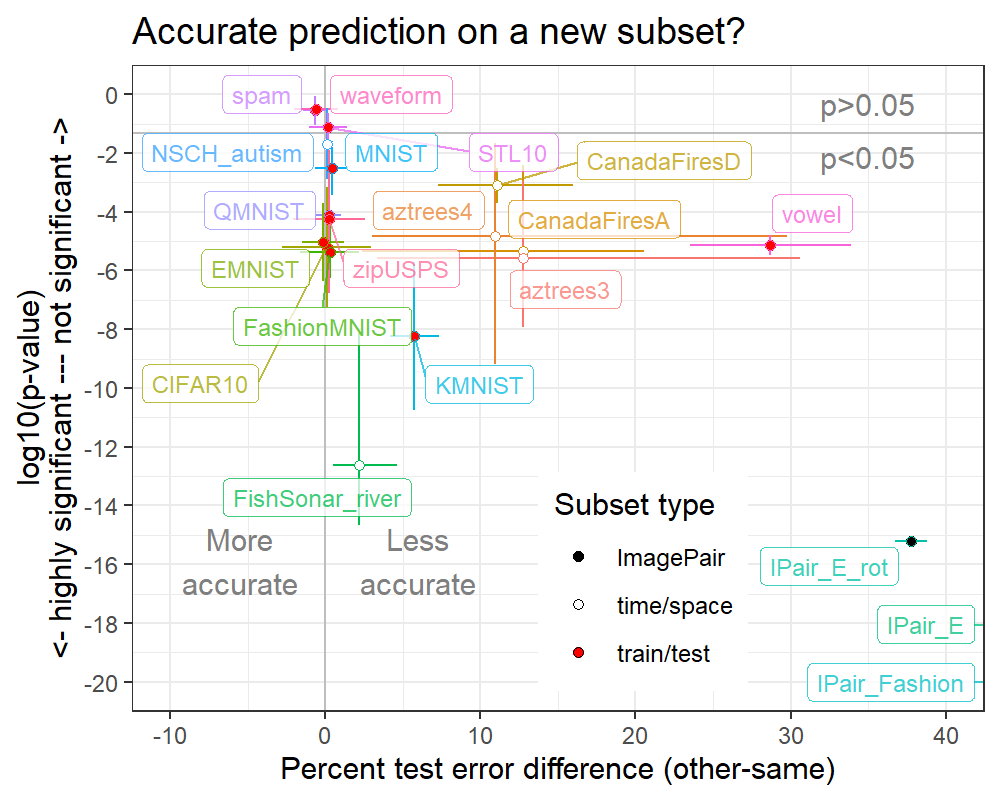
\includegraphics[height=\textheight]{data_Classif_batchmark_registry_scatter_other_segments.png} 
\end{frame}
 
\begin{frame}
  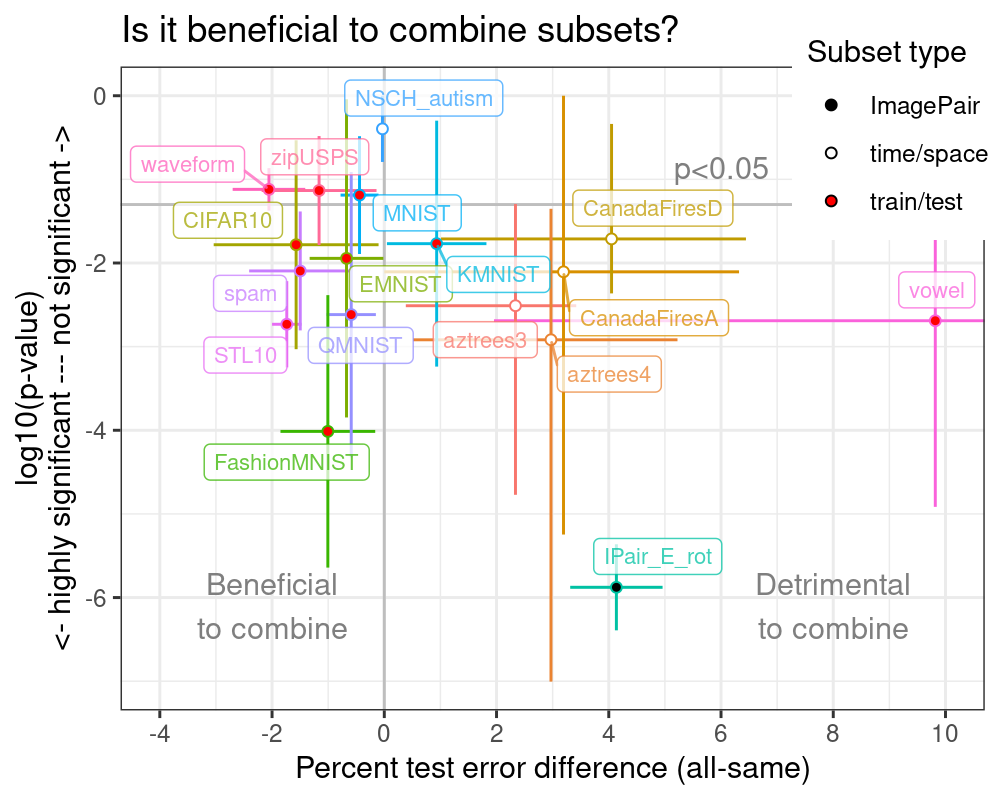
\includegraphics[height=\textheight]{data_Classif_batchmark_registry_scatter_all_segments.png}
\end{frame}
 
\begin{frame}
  \frametitle{Discussion and Conclusions}
  \begin{itemize}
  \item Proposed SOAK algorithm estimates similarity of
    learnable patterns between 
    subsets (space, time, etc).
  \item SOAK idea is new to ML frameworks\\
    (proposed \textbf{subset} column/idea not the same as \textbf{group}).
  \item Free/open-source R package available in mlr3 framework (easy
    parallelization over algorithms, data sets, train/test splits)
    \url{https://github.com/tdhock/mlr3resampling}
  \item Ran SOAK in parallel over 20 classification data sets, 10
    folds, 2--4 subsets, Same/Other/All (1200+ train/test splits).
  \item Train on MNIST, predict on FashionMNIST (impossible), predict
    on EMNIST (surprisingly difficult, both are digits).
  \item Most pre-defined train/test subsets in benchmark data
    are similar (STL10/waveform), some are not (KMNIST/vowel).
  \item We observed similarity between years in Autism data (slight benefit to combining years, predicting on new year works).
  \item In fires/trees/fish data, we observed
    significant differences between images/regions/rivers.
  \end{itemize}
\end{frame}


\section{How to deal with class imbalance? \\ AUM: Area Under Min(FPR,FNR), a new differentiable loss for ROC curve optimization (JMLR'23)} 

\begin{frame}
  \frametitle{Review of supervised binary classification}
  
  \begin{itemize}
  \item Given pairs of inputs $\mathbf x\in\mathbb R^p$ and outputs
    $y\in\{0,1\}$ can we learn a score 
    $f(\mathbf x)\in\mathbb R$, predict $y=1$ when $f(\mathbf x)>0$?
  \item Example: email, $\mathbf x =$bag of words, $y=$spam or not.
  \item Example: images. Jones {\it et al.} PNAS 2009.
    \parbox{2in}{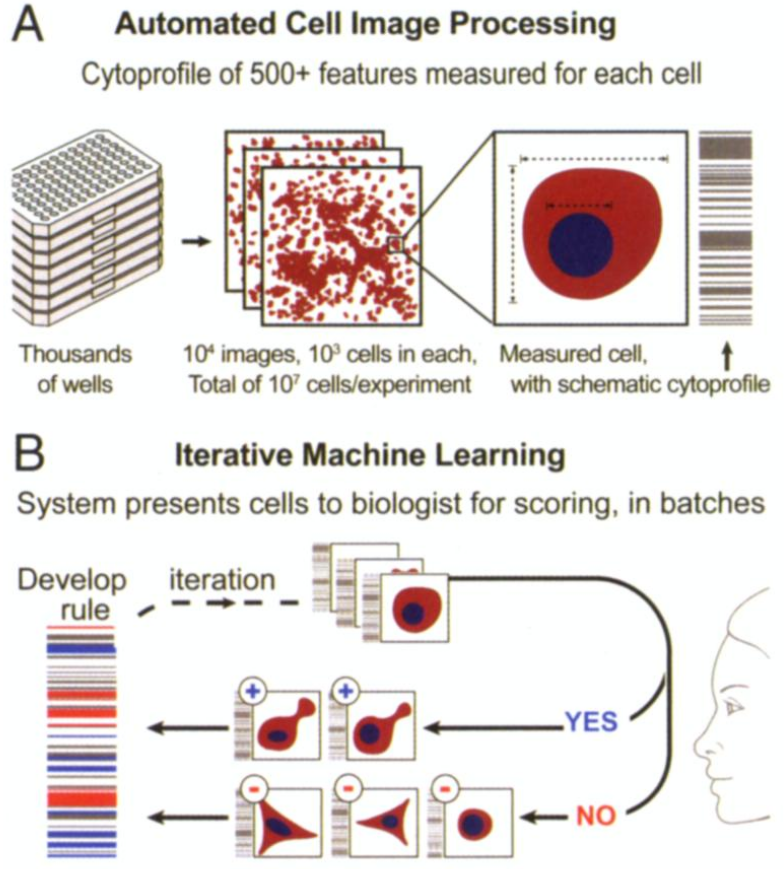
\includegraphics[width=2in]{cellprofiler}}
    \parbox{1.9in}{Gradient descent algorithms (Logistic regression, SVM, etc) minimize a differentiable surrogate of zero-one loss = sum of:\\
      \textbf{False positives:} $f(\mathbf x)>0$\\but $y=0$ (predict
      budding, but cell is not).\\
      \textbf{False negatives:} $f(\mathbf x)<0$\\but $y=1$ (predict
      not budding, but cell is).  }
  \end{itemize} 
\end{frame}

\begin{frame}
  \frametitle{ROC curves: fair comparison with different default FPR}

  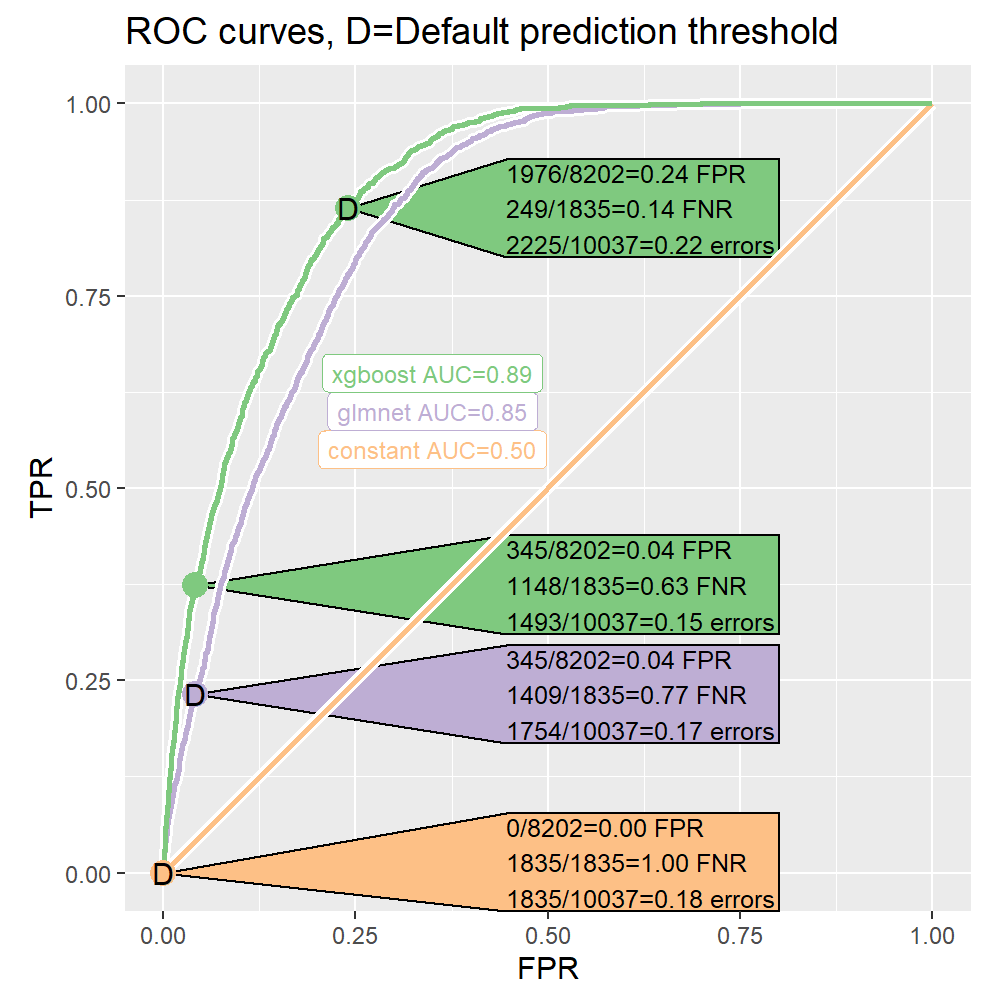
\includegraphics[width=0.65\textwidth]{figure-batchtools-expired-earth-roc}

  \begin{itemize}
  \item Imbalanced labels: 18\% positive, 82\% negative.
  \item At defaults (D), glmnet has fewer errors (misleading).
  \item At FPR=4\%, xgboost has fewer errors (fair comparison).
  \end{itemize}
\end{frame}

\begin{frame}
  \frametitle{Receiver Operating Characteristic (ROC) Curves}
  \begin{itemize}
  \item Classic evaluation method from the signal processing
    literature (Egan and Egan, 1975).
  \item ROC curve of learned $f$ is plot of True
    Positive Rate vs False Positive Rate: each point on the ROC curve
    is a different constant $c\in\mathbb R$ added to the predicted
    values: $f(\mathbf x)+c$.
  \item $c=\infty$ means always predict positive label (FPR=TPR=1).
  \item $c=-\infty$ means always predict negative label (FPR=TPR=0).
  \item Best classifier has a point near upper left (TPR=1, FPR=0), with large
    Area Under the Curve (AUC).
  % \item Proposed idea: a new surrogate for AUC that is differentiable,
  %   so can be used for gradient descent learning.
  \end{itemize}
  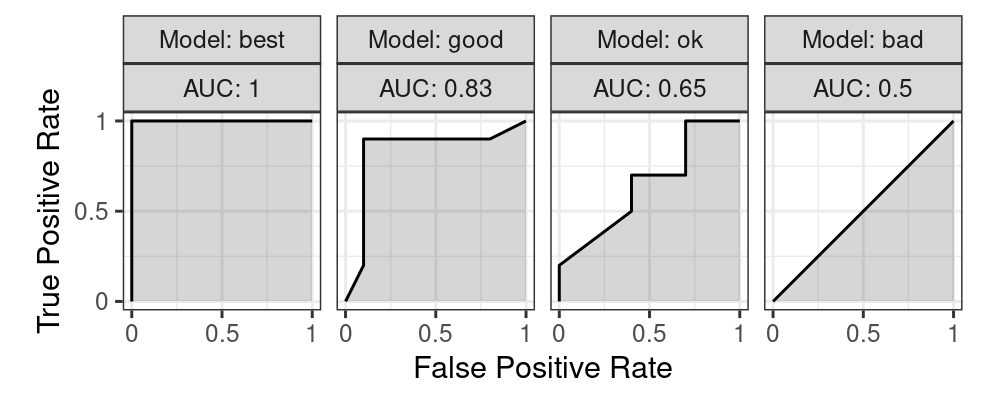
\includegraphics[width=\textwidth]{figure-more-than-one-new-binary}
\end{frame}



\begin{frame}
  \frametitle{Research question and new idea}
  Can we learn a binary classification function $f$ which directly
  optimizes the ROC curve?
  \begin{itemize}
  \item Most algorithms involve minimizing a differentiable surrogate
    of the zero-one loss, which is not the same.
  \item The Area Under the ROC Curve (AUC) is piecewise constant
    (gradient zero almost everywhere), so can not be used with
    gradient descent algorithms.
  \item We proposed (Hocking, Hillman 2023) to encourage points to be in the upper left of ROC
    space, using a loss function which is a differentiable surrogate
    of the sum of min(FPR,FNR).
  \end{itemize}
  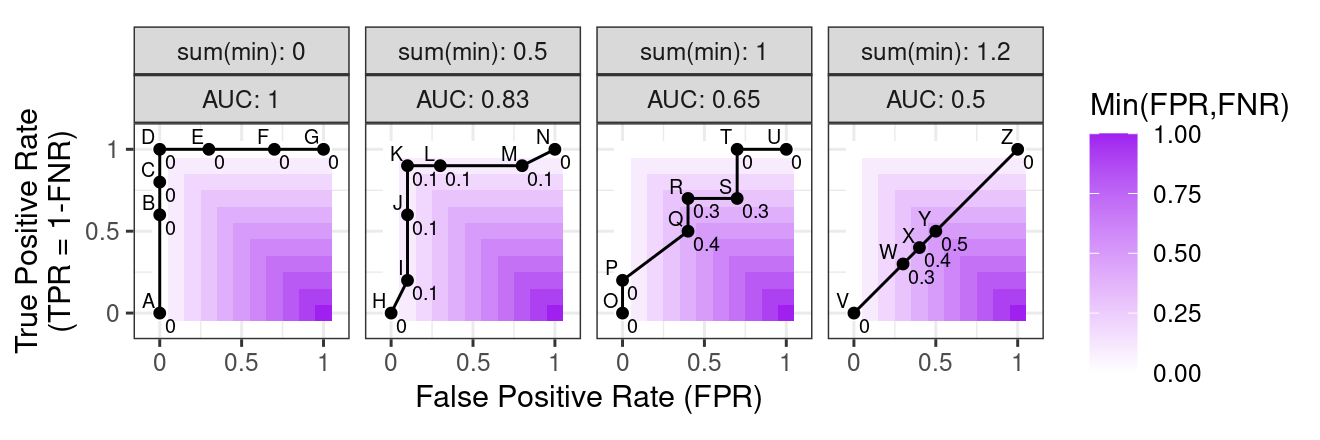
\includegraphics[width=\textwidth]{figure-more-than-one-new-binary-heat}
\end{frame}
 

\begin{frame}
  \frametitle{Comparing proposed loss with baselines}
  \begin{itemize}
  \small
  \item Classic baselines: hinge and logistic loss, sum over samples, $\ell[yf(x)]$.
  \item Bamber (1975) proved ROC-AUC relation to Mann-Whitney
    U statistic (double sum over all pairs of positive and negative
    samples).
  \item Recently:  $\text{SVM}^{\text{struct}}$ (Joachims 2005),
    X-risk (Yang 2022), %https://arxiv.org/abs/2206.00439
    All Pairs Squared Hinge (Rust and Hocking 2023),
    sum loss over pairs of positive and negative samples, $\ell[f(x^+)-f(x^-)]$.
  \item Proposed: sort-based AUM loss (sum over points on ROC curve).
  \item Figure below: loss for two samples: one positive, one negative.
  \end{itemize}

  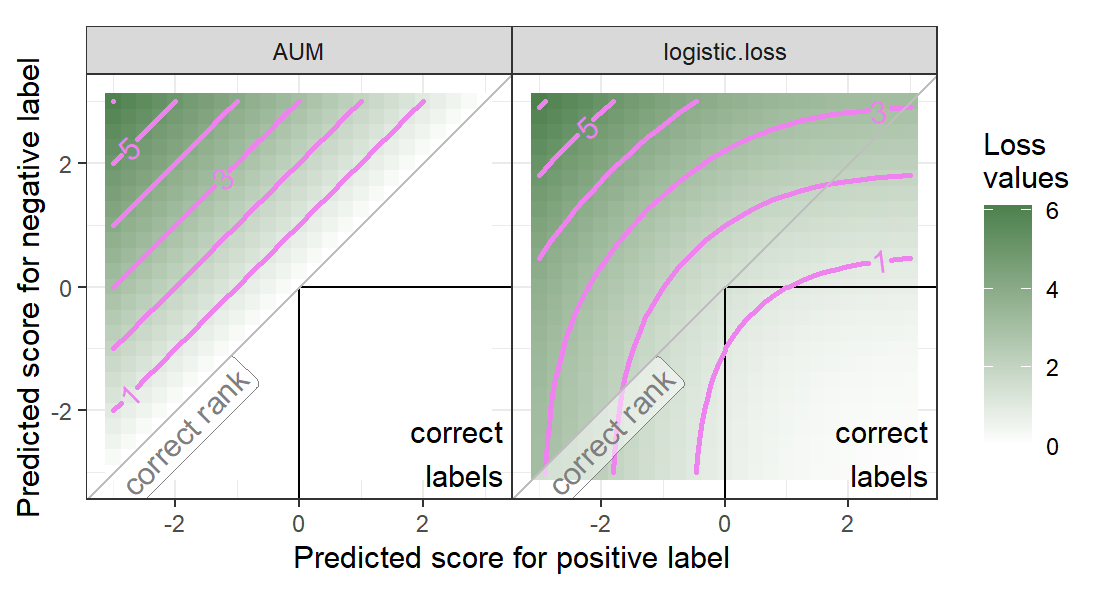
\includegraphics[width=0.7\textwidth]{figure-compare-hinge-loss-contours-logistic.png}

    Barr, Hocking, Morton, Thatcher, Shaw, \emph{TransAI} (2022).

  %AUM loss here = linear hinge with no margin, summed over pairs.
\end{frame}

\begin{frame}
  \frametitle{Large AUC $\approx$ small Area Under Min(FP,FN) (AUM)}
  \small
  
  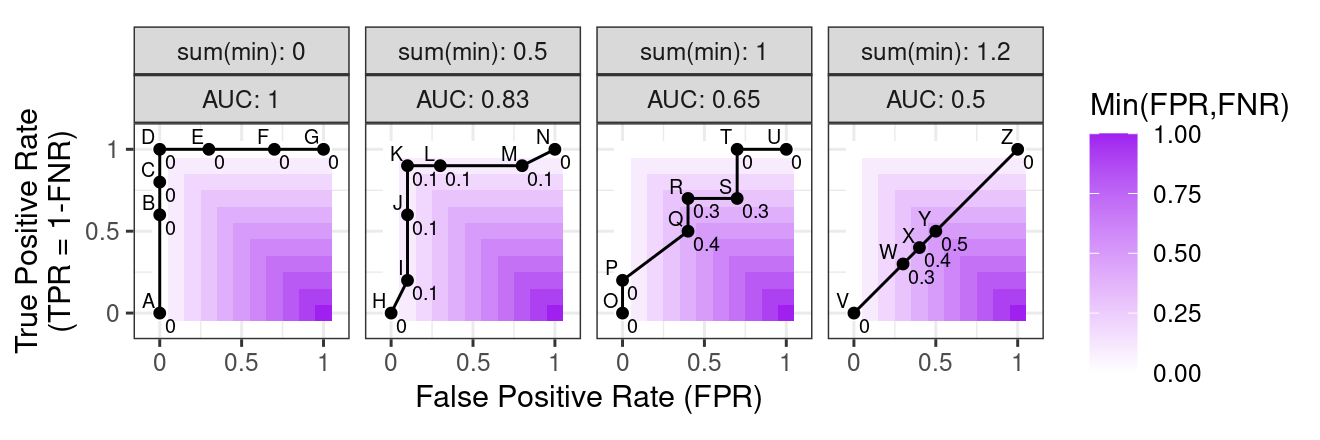
\includegraphics[height=1.3in]{figure-more-than-one-new-binary-heat}

  Above: purple heat map = numbers near dots = distance to top or left

  = same as black min error rate functions below.

  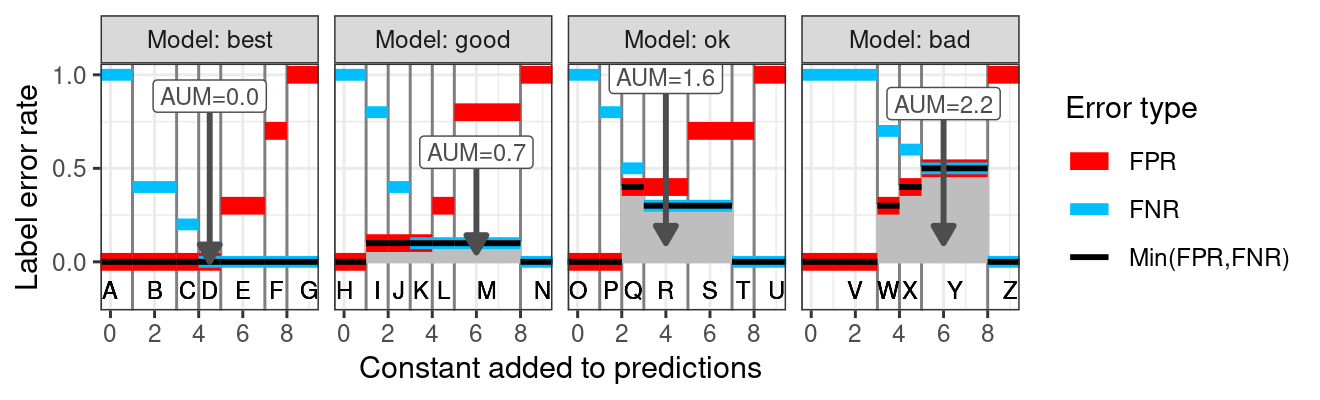
\includegraphics[height=1.3in]{figure-more-than-one-new-binary-aum-rate}

  Hocking, Hillman, \emph{Journal of Machine Learning Research} (2023).

  %Proposal: track how thresholds in error plot change with step size.
  
\end{frame}

\begin{frame}
  \frametitle{Computing Sum of Min (SM) over all ROC points}
  %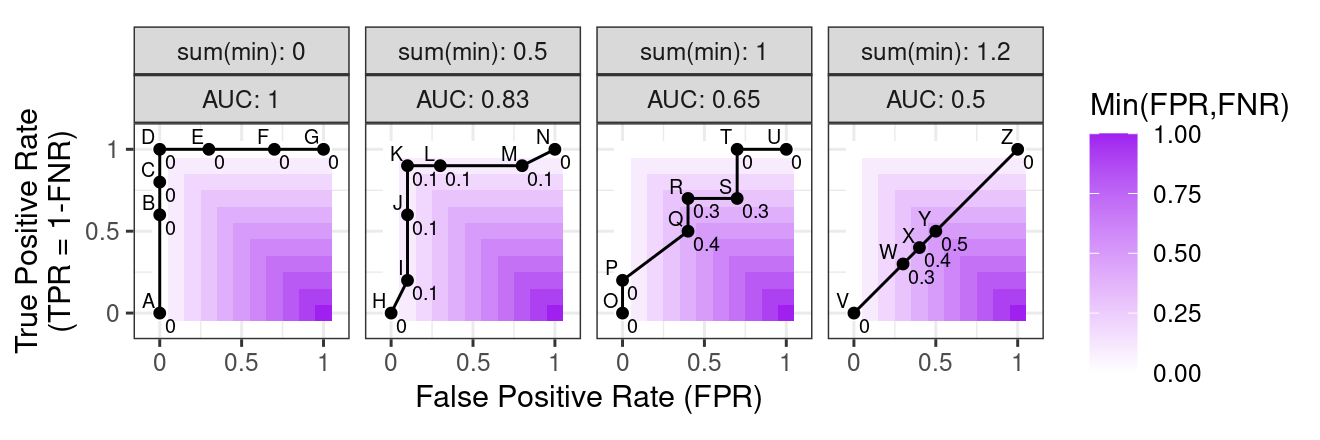
\includegraphics[width=\textwidth]{figure-more-than-one-new-binary-heat}
  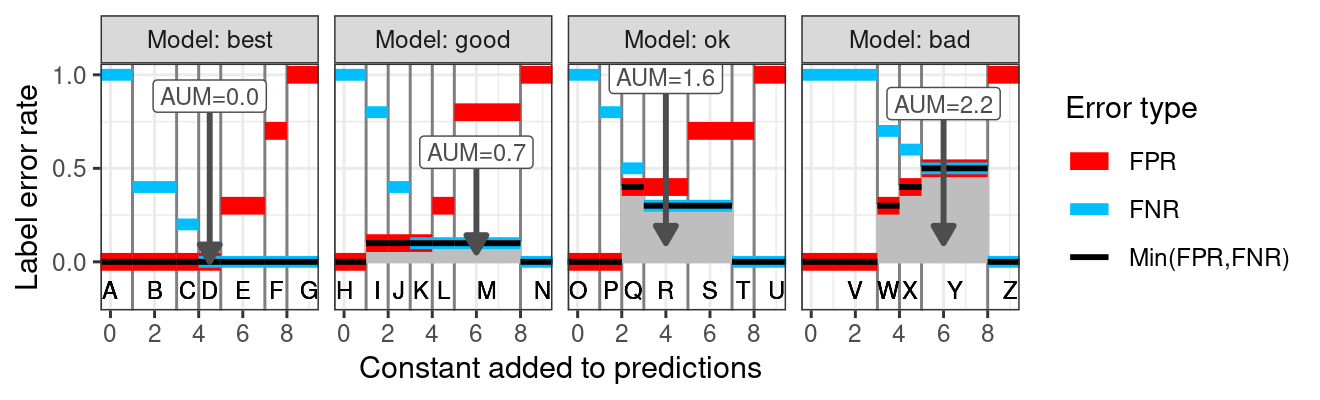
\includegraphics[width=\textwidth]{figure-more-than-one-new-binary-aum-rate}
  \vskip -0.2cm
  \begin{itemize}
  \item For $N$ samples, there are $\leq N+1$ points on the ROC curve,
  \item with sorted thresholds of $c$,  $T_1\leq\cdots\leq T_N\in\mathbb R$ (grey lines), 
  \item and corresponding min error values $M_2,\dots,M_N$ (black).
  \item Then if $I$ is the indicator function, we can write the sum of
    the min (SM), over all ROC points, as:
  \end{itemize}
\begin{equation*}
  \label{eq:SM-computation}
    \text{SM} =
    \sum_{i=2}^{N}
    I[ T_{i} \neq T_{i-1} ]
    M_i =
    \sum_{i:T_{i} \neq T_{i-1} }
    M_i.
\end{equation*}

($\neq$ required: a tie $T_i=T_{i-1}$ deletes a point from the ROC curve)

\end{frame}

\begin{frame}
  \frametitle{Computing proposed loss, Area Under Min (AUM)}
  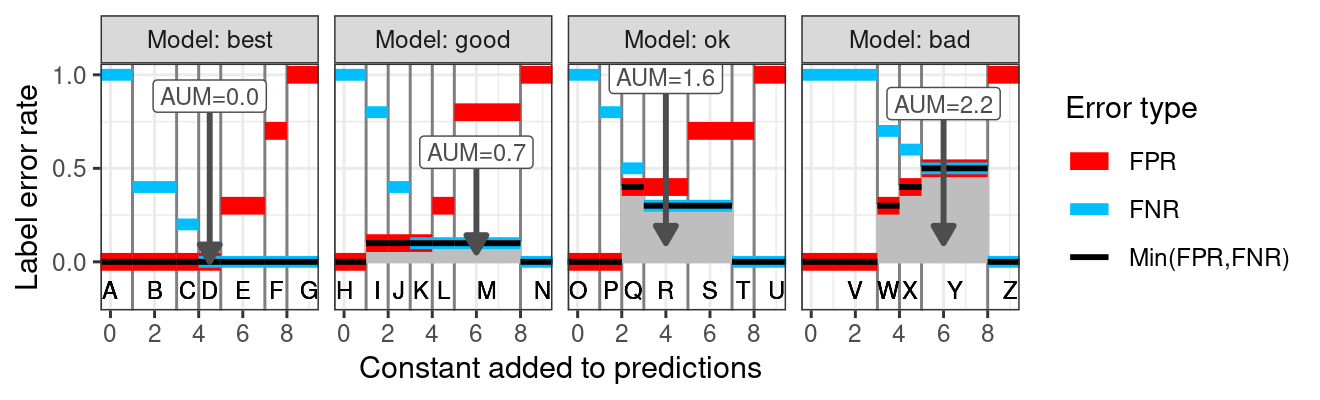
\includegraphics[width=\textwidth]{figure-more-than-one-new-binary-aum-rate}

The proposed AUM can be interpreted as an L1 relaxation of SM,
\vskip -0.5cm
\begin{eqnarray*}
  \text{(gradient zero) } \text{SM} &=&
    \sum_{i=2}^{N}
    \alert{\underbrace{I[ T_{i} \neq T_{i-1} ]}_{\text{L0}}}
    M_i =
    \sum_{i:T_{i} \neq T_{i-1} }
                  M_i.
                                    \\
  \text{(gradient non-zero) } \text{AUM} &=&
    \sum_{i=2}^{N}
    \alert{\underbrace{[ T_{i} - T_{i-1} ]}_{\text{L1}}}
                   M_i.\\
\end{eqnarray*}
\vskip -0.5cm

AUM is therefore a surrogate loss for ROC-SM minimization.\\
L1 relaxation $\Rightarrow$ constant/non-zero gradients.
\end{frame}

\begin{frame}[fragile]
  \frametitle{ROC curve pytorch code uses argsort}
\small
  \begin{verbatim}
def ROC_curve(pred_tensor, label_tensor):
  sorted_indices = torch.argsort(-pred_tensor)
  ... # torch.cumsum() etc
  return { # a dictionary of torch tensors
    "FPR":FPR, "FNR":FNR, "TPR":1 - FNR,
    "min(FPR,FNR)":torch.minimum(FPR, FNR),
    "min_constant":torch.cat([
      torch.tensor([-torch.inf]), uniq_thresh]),
    "max_constant":torch.cat([
      uniq_thresh, torch.tensor([torch.inf])])  }
>>> pd.DataFrame(ROC_curve(torch.tensor(
...   [2.0, -3.5, -1.0, 1.5]), torch.tensor([0,0,1,1])))
   FPR  FNR  TPR  min(FPR,FNR)  min_constant  max_constant
0  0.0  1.0  0.0           0.0          -inf          -2.0
1  0.5  1.0  0.0           0.5          -2.0          -1.5
2  0.5  0.5  0.5           0.5          -1.5           1.0
3  0.5  0.0  1.0           0.0           1.0           3.5
4  1.0  0.0  1.0           0.0           3.5           inf
\end{verbatim}

    \url{https://tdhock.github.io/blog/2024/torch-roc-aum/}

\end{frame}


\begin{frame}[fragile]
  \frametitle{AUC and proposed AUM both use ROC curve}

  \begin{verbatim}
def ROC_AUC(pred_tensor, label_tensor):
    "Classic metric, but gradient zero almost everywhere"
    roc = ROC_curve(pred_tensor, label_tensor)
    FPR_diff = roc["FPR"][1:]-roc["FPR"][:-1]
    TPR_sum = roc["TPR"][1:]+roc["TPR"][:-1]
    return torch.sum(FPR_diff*TPR_sum/2.0)

def Proposed_AUM(pred_tensor, label_tensor):
    "Surrogate loss, non-zero gradient for predictions"
    roc = ROC_curve(pred_tensor, label_tensor)
    min_FPR_FNR = roc["min(FPR,FNR)"][1:-1]
    constant_diff = roc["min_constant"][1:].diff()
    return torch.sum(min_FPR_FNR * constant_diff)
\end{verbatim}

  \url{https://tdhock.github.io/blog/2024/torch-roc-aum/}
\end{frame}

\begin{frame}[fragile]
  \frametitle{Proposed AUM pytorch code, auto-grad demo}

  \begin{itemize}
  \item Assume two samples, $(x_0,y_0=0), (x_1,y_1=1)$,
  \item Plot objective and gradient with respect to predicted scores.
  \end{itemize}

  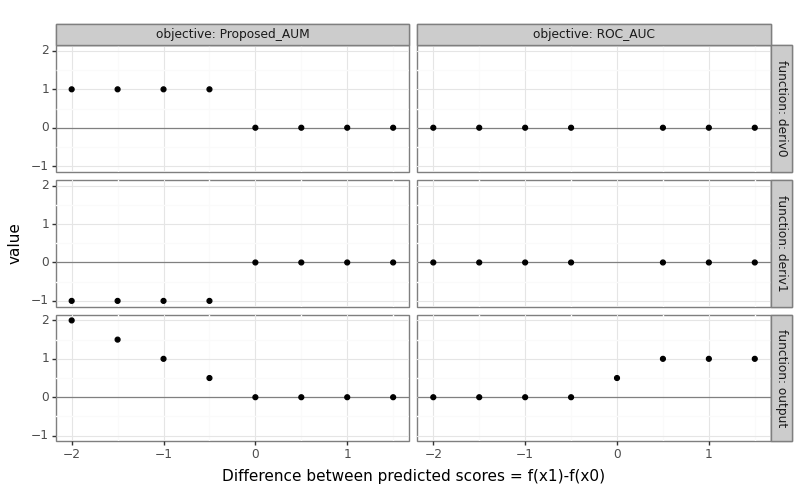
\includegraphics[width=\textwidth]{gg_aum_grad}

  \url{https://tdhock.github.io/blog/2024/torch-roc-aum/}
\end{frame}

\begin{frame}
  \frametitle{Comparing proposed AUM with weighted logistic loss}
  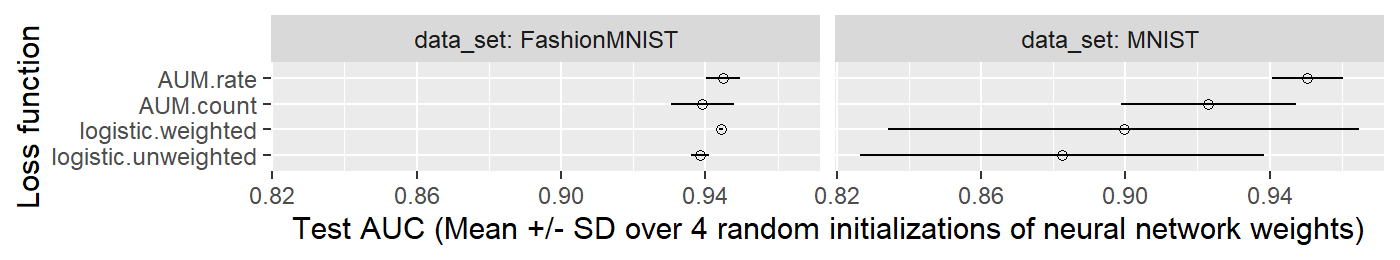
\includegraphics[width=\textwidth]{figure-aum-neural-networks-test-auc}
  \begin{itemize}
  \item Image classification data sets (0--4=negative, 5--9 positive).
  \item Train set 1\% positive, test set balanced.
  \item LeNet5 convolutional neural network, batch size 1000.
  \item Step size from $10^{-4}$ to $10^2$ (keep best).
  \item AUM rate uses Area Under Min of FPR/FNR, more accurate in
    these data than AUM count (FP/FN totals).
  \item logistic unweighted is usual binary cross-entropy loss (uniform weight=1 for each sample). 
  \item for logistic weighted, we compute class frequencies, $n_1=\sum_{i=1}^N I[y_i=1]$ and $n_0$ similar; then weights are $w_i=1/n_{y_i}$ so that total weight of positive class equals total weight of negative class (more accurate in these data).
  \end{itemize}
\end{frame}

\begin{frame}
  \frametitle{AUM gradient descent increases validation AUC,\\
    four image classification data sets}
 
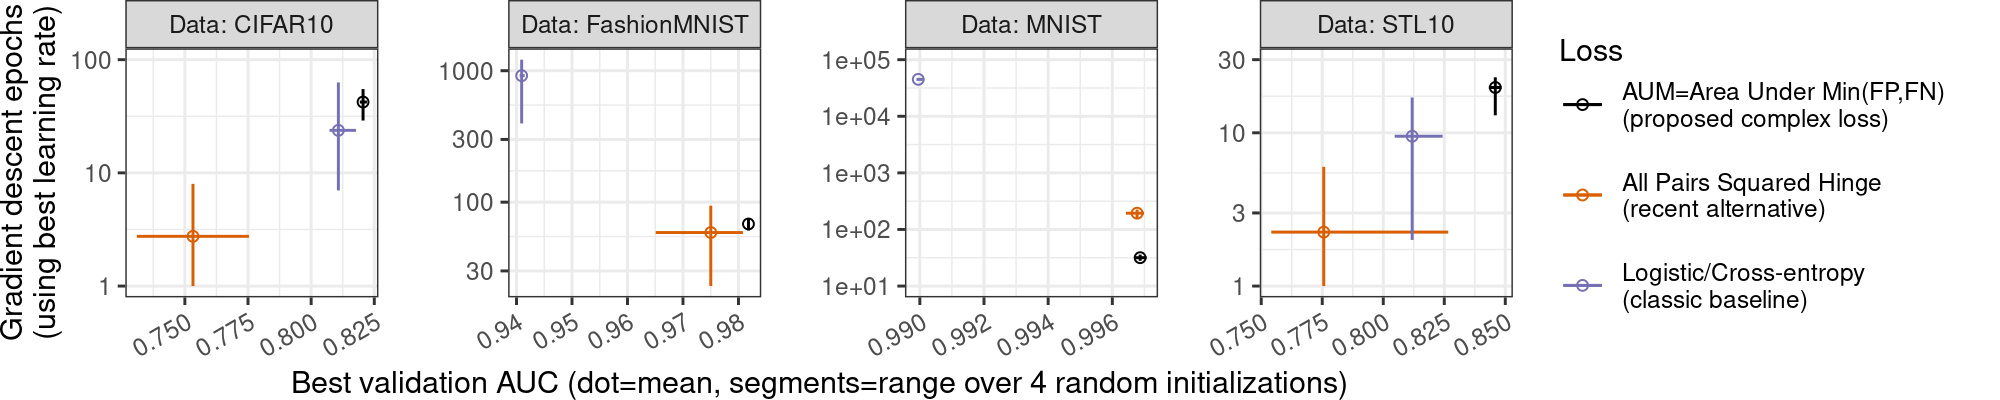
\includegraphics[width=\textwidth]{data_Classif_batchtools_best_valid_scatter}

\begin{itemize}
\item Unbalanced binary classification: 10\% negative, 90\% positive.
\item Gradient descent with constant step size, best of $10^{-4}$ to $10^5$.
\item Full gradient (batch size = number of samples).
\item Linear model, max iterations = 100,000.
\item Max Validation AUC comparable or better than baselines: logistic loss and all paired squared hinge.
\item Number of epochs comparable to baselines.
\item AUM time per epoch is $O(N \log N)$ (sort), small log factor larger than standard logistic/cross-entropy loss, $O(N)$.
\end{itemize}

\end{frame}

\begin{frame}
  \frametitle{Discussion and future work}
  \begin{itemize}
  \item Classic classification losses are L1 relaxations of the zero-one loss, defined as a sum over samples.
  % \item Proposed AUM loss similar to recent all pairs losses\\
  %   (minimal for predicted scores with correct ranks,\\
  %   can be implemented by sorting predicted scores).
  \item Proposed AUM loss is an L1 relaxation defined as a sum over
    points on the ROC curve (requires sorting predicted scores).
  \item Proposed AUM loss can be used in gradient descent instead of logistic/binary cross-entropy loss. PyTorch code: \url{https://tdhock.github.io/blog/2024/torch-roc-aum/}
  \item Best use with stochastic gradient algorithms?
    At least one positive and one negative example is required in each
    batch.
  \item Algorithms like SVM? (margin/kernel)
  \item How to adapt to multi-class setting, and other problems such as
    ranking/information retrieval?
  \item See our JMLR'23 paper for an application to supervised
    change-point detection, and arXiv:2410.08635 for an efficient line
    search that exploits the piecewise linear/constant nature of
    AUM/AUC.
  \end{itemize}
\end{frame}

\begin{frame}
  Thanks! Please email me if you are interested to collaborate: toby.dylan.hocking@usherbrooke.ca

  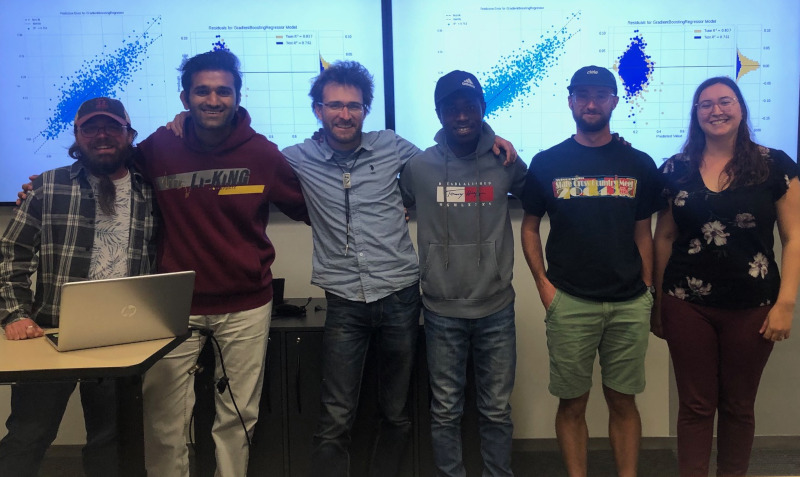
\includegraphics[width=\textwidth]{2022-10-14_ML_group_meeting}

  Reproducible slide/figure source code: \url{https://github.com/tdhock/cv-same-other-paper} \url{https://github.com/tdhock/max-generalized-auc}
\end{frame}

\begin{frame}
  \frametitle{Gradients of sample-based loss are influenced by imbalance}
  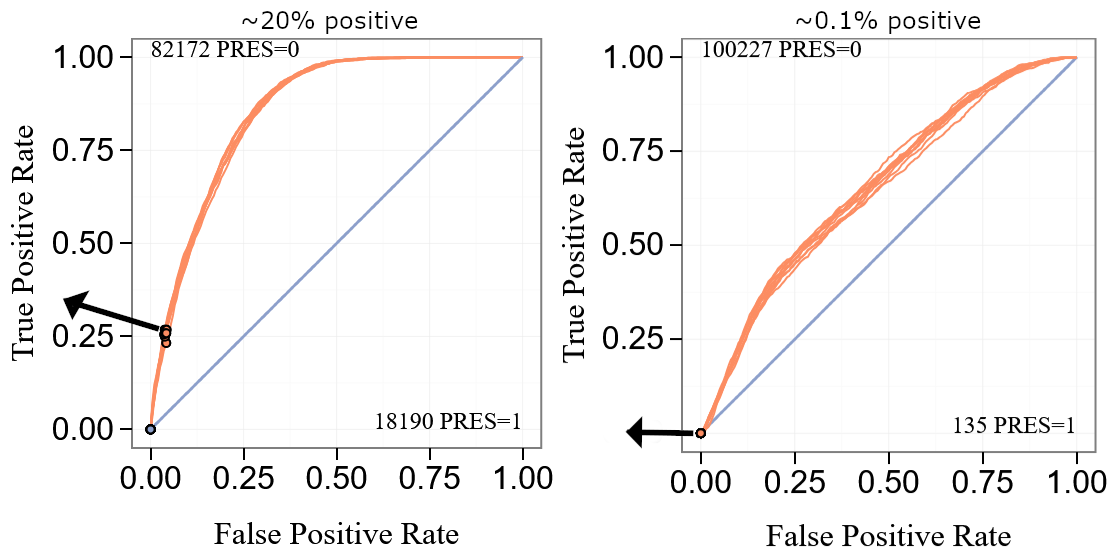
\includegraphics[width=\textwidth]{roc-gradient-arrows}
  \begin{itemize}
  \item Left: some imbalance, ~20\% positive labels, gradient 4x
    stronger along X axis / False Positive Rate.
  \item Right: large imbalance, ~0.1\% positive labels, gradient 1000x
    stronger along X axis / False Positive Rate. (True Positive / Y
    axis gradients essentially ignored)
  \end{itemize}
\end{frame}

\begin{frame}
  \frametitle{Gradients using balanced sample weights, proposed loss}
  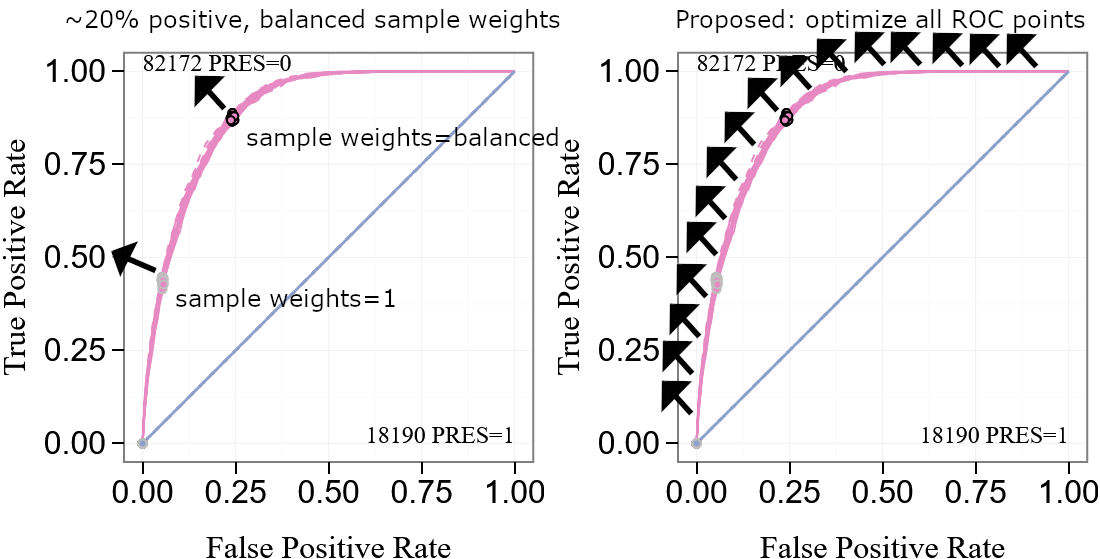
\includegraphics[width=\textwidth]{roc-gradient-arrows-proposed}
  \begin{itemize}
  \item Left: gradient 4x
    stronger along X axis for sample weights=1. Balanced sample
    weights mean equal influence for gradients along both axes, based on the current prediction threshold.
  \item Right: proposed method computes gradients based on all ROC
    points, not just the current prediction threshold.
  \end{itemize}
\end{frame}

\end{document} 
